\FloatBarrier
\subsection{Mechanics of the suspension upper stages }
\label{sec:Upper_stages_mechanics}
%\emph{
%Author(s): S.\ Braccini, F.\ Frasconi}
\FloatBarrier
\subsubsection{LF interferometer}

In this paragraph we discuss in details the problem of the attenuation of the seismic noise  and we present  a possible solution for both ET-LF and ET-Hf interferometers.  The focus is set on a Virgo {\emph {Superattenuator}} solution. In fact, it has been experimentally demonstrated \cite{Collaboration2010} that this solution provides already a seismic noise attenuation of  more than ten order of magnitude starting from a few Hertz.  Alternative approaches are cited in the Appendix, where the geometric anti-spring and the active filter developed in LIGO, GEO, TAMA  and at the NIKHEF laboratory are  described. The material compatibility of the \emph{Superattenuator} with a cryogenic environment is discussed also there.
In the following we will present in sequence

\begin{itemize}
\item  The ET attenuation requirements
\item The Virgo Superattenuator
\item Seismic isolation measurements with the Superattenuator (SA)
\item SA modifications for Low Frequency ET
\item Noise from SA mechanical micro-glitches
\item SA control strategy and improvements for ET
\end{itemize}

\paragraph{a) Attenuation Requirements} 

As shown in figure~\ref{FigSusp1}, Virgo is operating close to its design sensitivity also in the low frequency range. Looking at the detector noise budget, it turns out that its response is not limited by the mirror seismic noise passing through the anti-seismic suspension (\emph{Superattenuators}). A set of measurements aimed to check if the present \emph{Superattenuator} performance is compliant with the higher sensitivity of the next generation antennae, in particular with the Einstein Telescope, has been performed. 
The mechanical transfer function requirements for seismic noise isolation of the mirror in future detectors can be obtained starting from their design sensitivity curve expressed in terms of the mirror displacement. To this purpose, in figure~\ref{FigSusp2}, the design sensitivity curves of Advanced Virgo~\cite{AdV2009}, the upgraded 3\,km-long interferometer expected to enter in action in 2014 at the Virgo site, and those ones for the two reference solutions of the Einstein Telescope, are compared.
%   
\begin{figure}[t!]
	\begin{center}
		 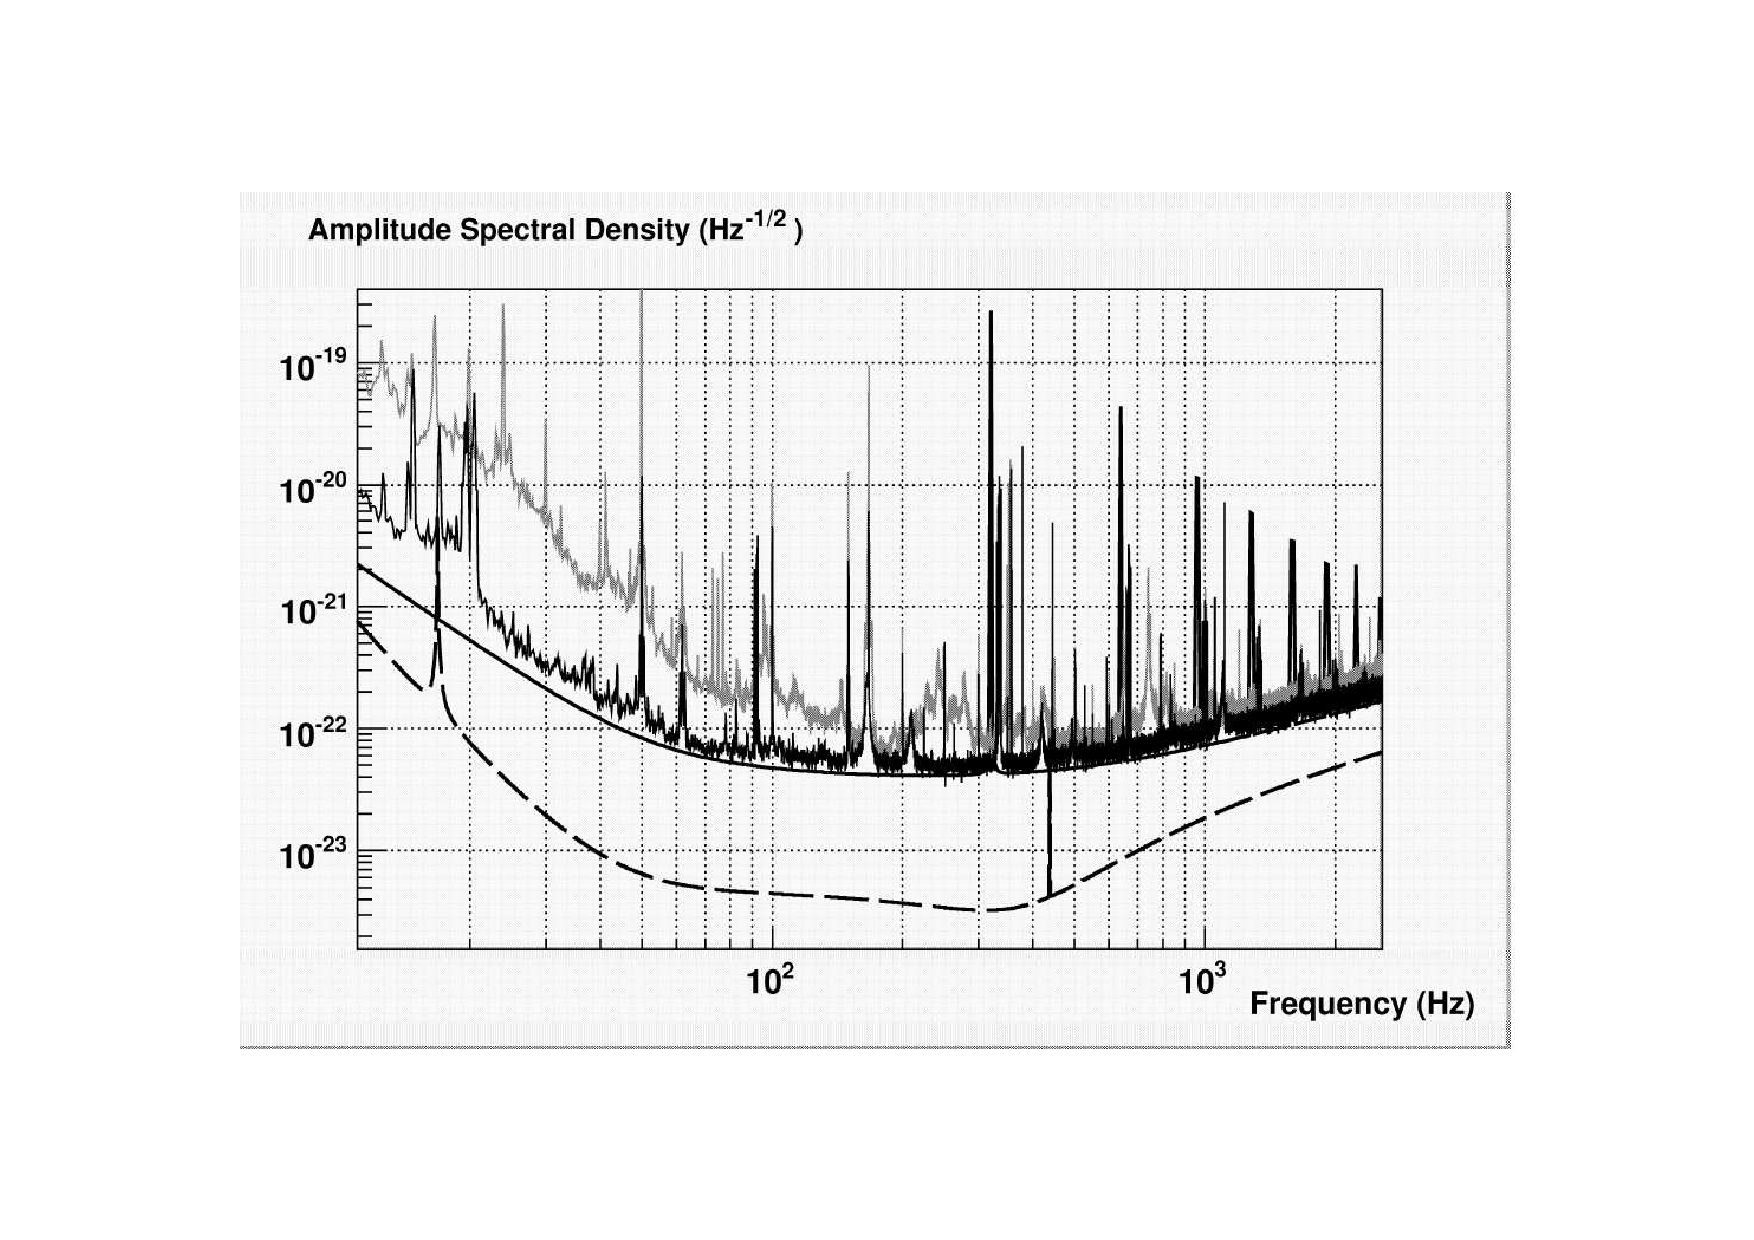
\includegraphics[width=18cm]{./Sec_Suspensions/Figures/Fig1.pdf}
			\caption{Virgo sensitivity achieved after a few months of the second   scientific run (\emph{VSR2} - black experimental curve), compared with the sensitivity reached in 2007 during the first scientific run (\emph{VSR1} - grey curve). The continuous curve is the Virgo design sensitivity, discussed in \cite{Punturo2004}, while the dotted curve is the design sensitivity of Advanced Virgo, the next generation detector.}
\label{FigSusp1}
	\end{center}
\end{figure}
%
\begin{figure}[t!]
	\begin{center}
		 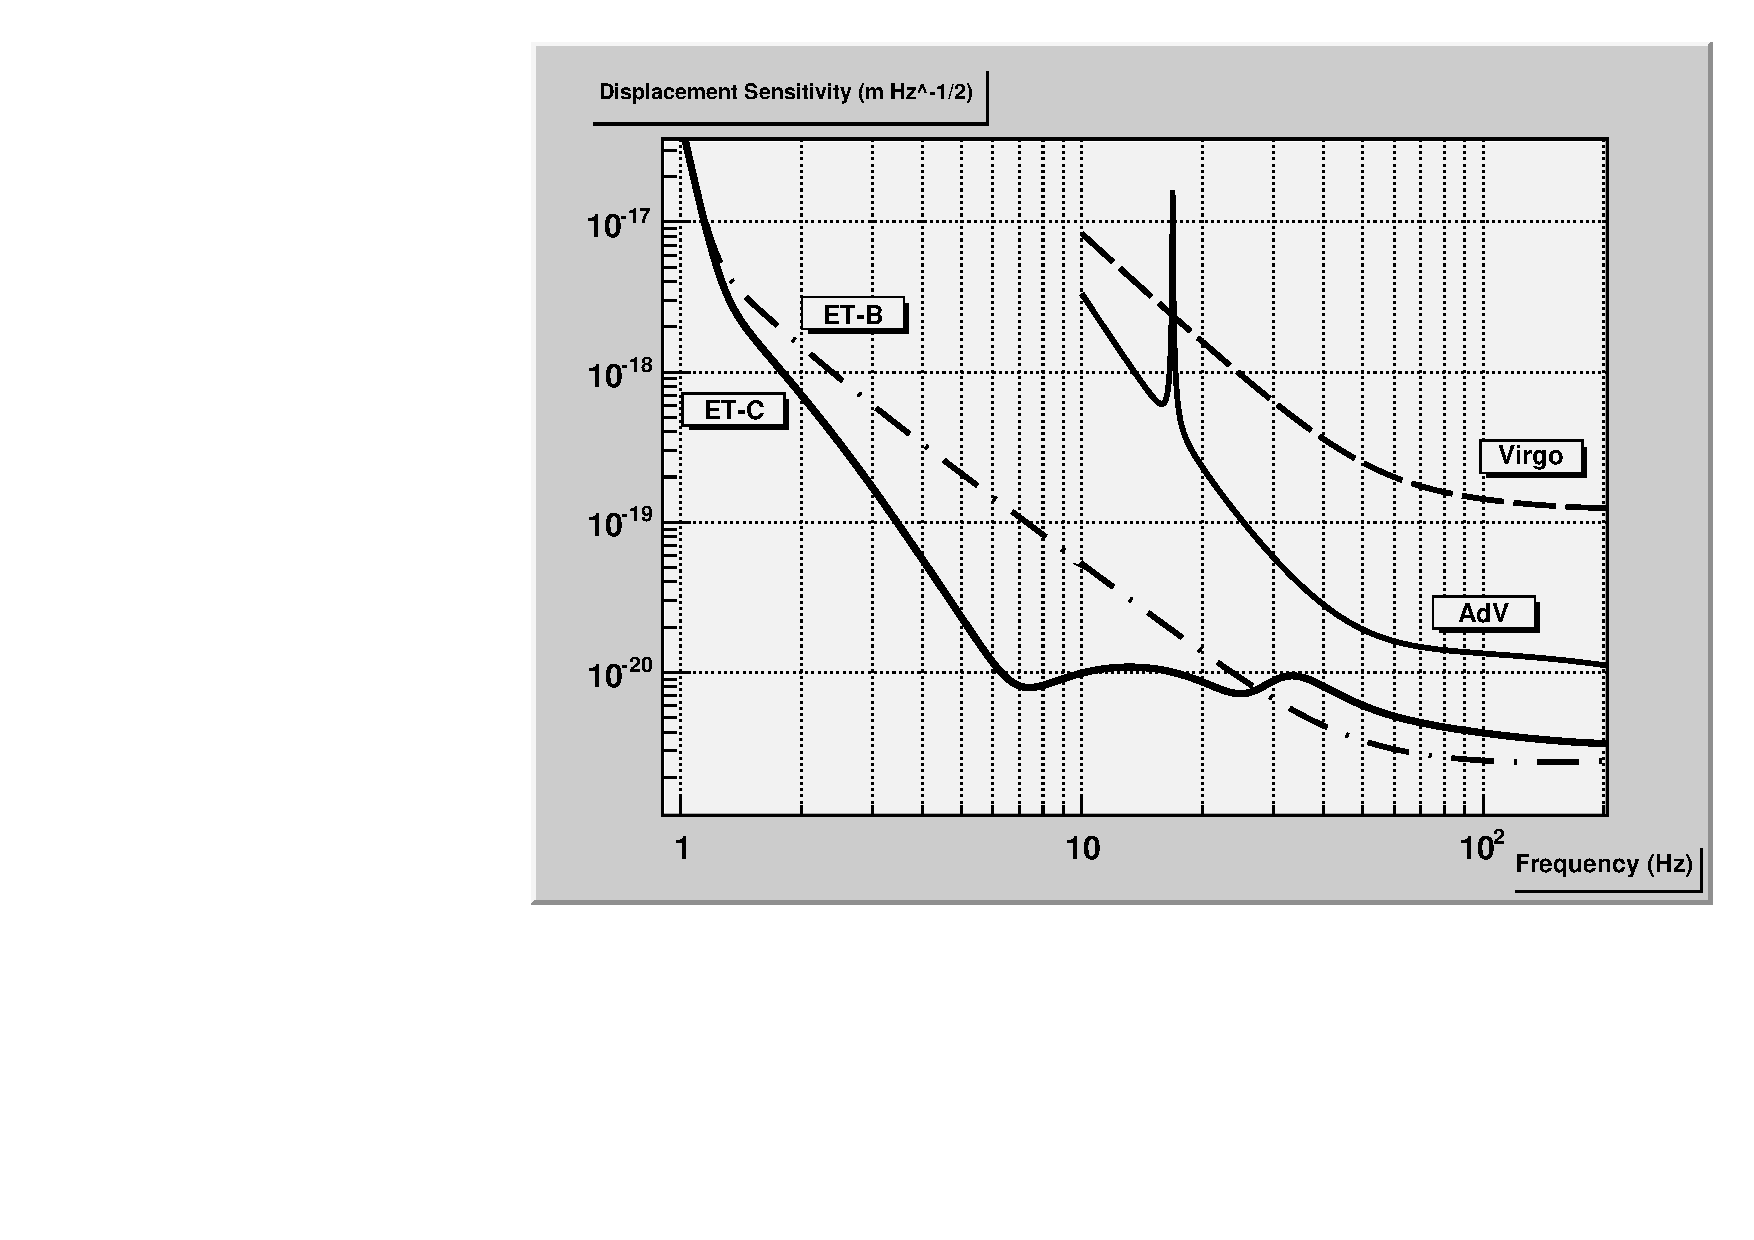
\includegraphics[width=16cm]{./Sec_Suspensions/Figures/Fig2.pdf}
			\caption{Displacement design sensitivities of Virgo, Advanced Virgo~(AdV), and of the two reference configurations of the Einstein Telescope: the high-frequency interferometer (ET-B) and the `xylophone' design (ET-C), optimized for the low frequency detection. While the detection bandwidth of Virgo and AdV starts from 10 Hz, Einstein Telescope aims to extend the detection bandwidth in the low frequency region starting from a few Hz.}
\label{FigSusp2}
	\end{center}
\end{figure}
%
\begin{figure}[t!]
	\begin{center}
		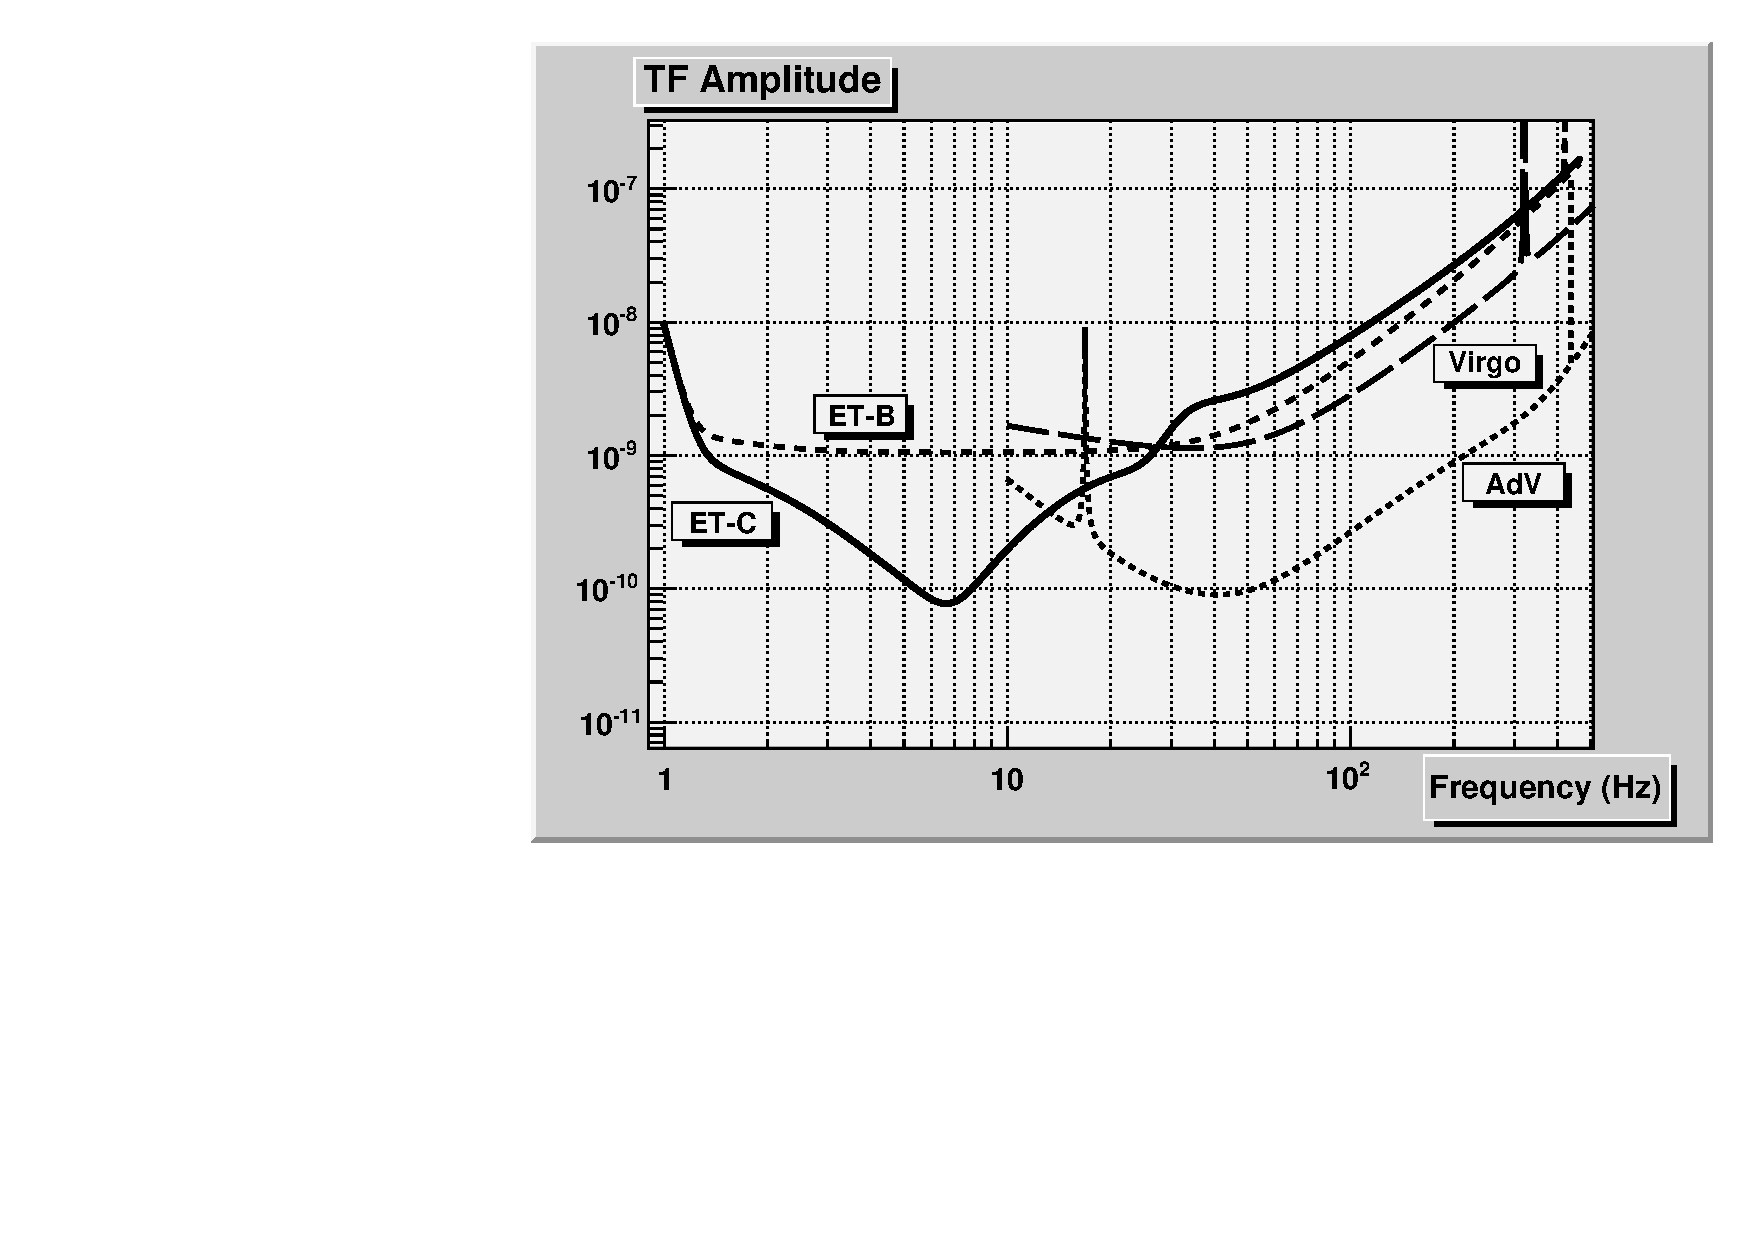
\includegraphics[width=16cm]{./Sec_Suspensions/Figures/Fig3.pdf}
			\caption{Seismic vibration transfer function requirements for different antennas. The curves represent the ratio between the displacement sensitivities reported in figure~\ref{FigSusp2} and the conservative linear spectral density of seismic noise at the level where the interferometer is located. Since seismic noise will be at least a couple of orders of magnitude smaller in underground environment, Einstein Telescope, despite its better sensitivity, is less demanding in terms of seismic attenuation at high frequency.}
\label{FigSusp3}
	\end{center}
\end{figure}
%
The maximum acceptable transfer function amplitude of the seismic isolation system in different antennas is plotted as a function of the frequency in figure~\ref{FigSusp3}. This is given by the ratio between the detector displacement sensitivity curves reported in figure~\ref{FigSusp2} and the linear spectral density of seismic noise measured on site at ground level. At the Advanced Virgo site (the same of Virgo) the linear spectral density of the ground seismic displacement has been measured to be roughly isotropic and well approximated, between a fraction of Hz and a few tens of Hz, by the function $A/f^{2}$, where $f$ indicates the spectral frequency and $A$ is around $10^{-7}\,\mathrm{m\cdot Hz^{3/2}}$~\cite{Acernese2004}. A conservative value of $A$ around $5\times10^{-7}\,\mathrm{m\cdot Hz^{3/2}}$ has been considered to take into account possible fluctuations in some spectral regions, and the fact that the residual displacement due to seismic noise affects all four mirrors of the two Fabry-Perot cavities. Since the Einstein Telescope site has not yet been chosen, the requirement has to be considered as provisional. The linear spectral density seismic noise of $5\times 10^{-9}/f^{2}$, measured in the Kamioka mine, where the new cryogenic Japanese interferometric detector is planned to be installed~\cite{Ohashi2003July31-August7}, is taken as a reference value. The recent progresses of Einstein Telescope working group for site selection are promising~\cite{Beker2009}. In particular, a measurements campaign of seismic noise for different underground sites in Germany provides seismic spectra smaller by a few units or comparable with that one measured in Kamioka mine. This makes the chosen reference seismic floor conservative for our goals (the requirements are likely more stringent than necessary).

It is important to stress that the transfer function requirements are valid both for vertical and horizontal seismic noise, that have a similar magnitudes. While for horizontal direction the argument is straightforward, in the vertical case the plot represents the maximum fraction of vertical seismic noise that can be transferred to the mirror along the beam direction without affecting the antenna sensitivity. As shown in the following section, only a fraction of the mirror vertical motion is transmitted along the beam because of unavoidable mechanical coupling and Earth curvature (making 10\,km far plumb lines \footnote{A plumb line is  regarded as directed exactly toward the earth's center of gravity.} not parallel each other). 

\paragraph{b) The Virgo Superattenuator (SA)}

Since it will be shown that the \emph{Superattenuator} as it is operating within the Virgo interferometer is already compliant with the ET project requirements above 3\,Hz, it is important to provide a detailed description of the apparatus.
The \emph{Superattenuator} working principle is based on a simple idea. Exciting in horizontal direction the suspension point of a simple pendulum at frequency $f$ higher than the pendulum normal mode $f_0$, it is easy to prove that the oscillation is transmitted to the suspended mass with an attenuation proportional to $(f_0/f)^{2}$. Therefore a device suspending a mirror based on the working principle of a simple pendulum, represents a good isolation system for seismic noise at frequency $f > f_0$.
A better attenuation performance is achievable considering a \emph{n-stage} pendulum. With this system an oscillation at a frequency $f$ higher than the frequencies of the chain normal modes $(f>f_0>f_1> \ldots >f_n)$, is transmitted to the suspended mass with attenuation proportional to $f^{-2n}$. In particular, the ratio between the linear spectral density of the last mass displacement (the optical component) and the linear spectral density of the suspension point displacement (where the excitation is applied), decreases as $A/f^{2n}$ where 
$A=f_0^{2}\cdot f_1^{2} \cdot f_2^{2} \cdots f_n^{2}$ and $n$ is the number of stages. In this way a very large attenuation of seismic noise horizontal component can be obtained in the frequency range above the highest pendulum resonance, simply increasing the number of stages. The longer are the pendulums, the lower are the resonant frequencies of the system and higher is the attenuation response at a given frequency.

Unfortunately, due to different directions of the plumb line on the curved Earth surface, the end mirrors, suspended 3\,km away in the Virgo interferometer and 10\,km in Einstein Telescope, are misaligned (each with respect to the other) by about $3\times 10^{-4}$\,rad and $10\times 10^{-4}$\,rad respectively. For this reason it is necessary to tilt one mirror with respect to the other by the same amount, making at least one mirror misaligned with respect to the local plumb line. With this setting up the mirrors are not perfectly perpendicular to the laser beam and then any vertical vibration will be partially transmitted to the interferometer horizontal axis (laser beam direction). In addition any vertical vibration will be partially transmitted to the interferometer horizontal axis because of an unavoidable coupling among different degrees of freedom. Thus vertical motion will cause a phase change of the laser beam. It is thus clear that a vertical attenuation of seismic noise comparable with the horizontal one is fundamental to reduce the observation frequency threshold. With a multistage pendulum this goal can be achieved by replacing each suspension wire with a spring to form a cascade of oscillators also along the vertical direction. The spring should support a heavy load and, at the same time, it should be soft enough to exhibit a low resonant frequency. With this technical solution it is possible to confine the vertical resonances of the chain in a low frequency range obtaining a strong attenuation starting from a few Hz. 

Even the unavoidable mechanical couplings between rotations and horizontal beam direction can cause a phase change on the interferometer laser beam. In order to confine these rotational mode frequencies well below the detection band, each pendulum mass has to be replaced by a structure having a high momentum of inertia. In addition, the diameter of the suspension wire, connecting two consecutive stages, has to be small enough to reduce its restoring torque which opposes the rotation of the chain and determining its rotational frequencies. An interconnection of the stages at small distance and as close as possible to their centres of mass, guarantees low frequency tilt modes (i.e.\ rotational modes around the two horizontal axes) and a negligible coupling effects on the horizontal displacement of the suspended mass.

Keeping in mind all the considerations reported above, the Virgo \emph{Superattenuator} has been conceived having a mechanical structure based on the working principle of a multistage pendulum~\cite{Ballardin2001}. Each mirror, indeed, is suspended to a 8\,m-long SA chain with 6 mechanical filters (see Fig.~\ref{SAfig1}). The system consists of three fundamental elements: the Inverted Pendulum (\emph{IP}), the mechanical seismic Filters (\emph{SF}) connected each other by metallic suspension wires and the Last Stage (\emph{LS}) or optical payload. The suspension system is described here below, while more detailed information of each single chain element can be found in reference~\cite{TheVirgoCollaboration1995}.

\begin{figure}[t]
	\begin{center}
		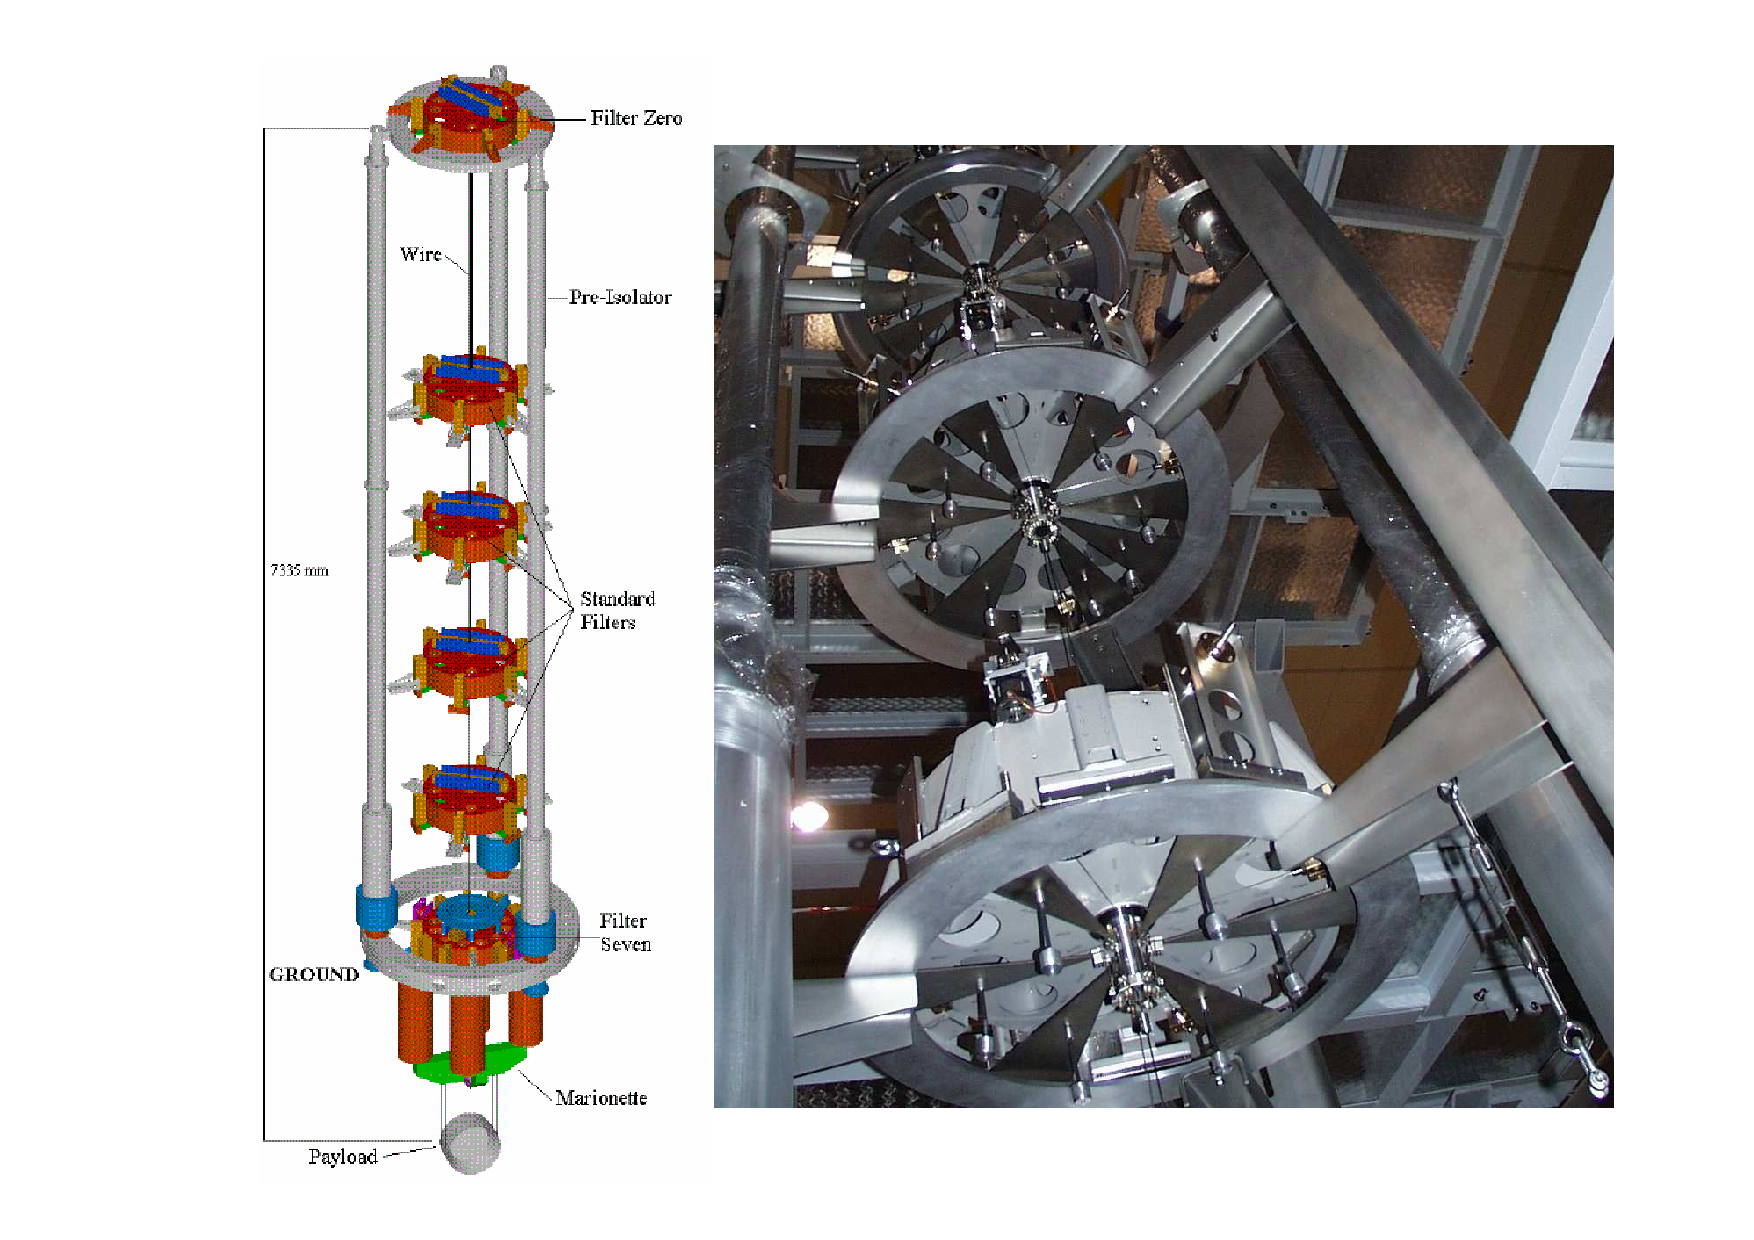
\includegraphics[width=17cm]{./Sec_Suspensions/Figures/SAfig1.pdf}
			\caption{The Virgo \emph{Superattenuator} suppresses the transmission of ground seismic vibrations to the suspended mirror. The mechanical filter chain and the three legs of the inverted pendulum are visible. In our attenuation measurements the excitation is applied to the filter chain suspension point.}
\label{SAfig1}
	\end{center}
\end{figure}

\subparagraph{The Inverted Pendulum top stage}
The top stage of the \emph{Superattenuator} is designed to fulfil three main functions:
\begin{itemize}
\item to introduce a very low frequency (about 40\,mHz) horizontal filtering stage, limiting the amount of seismic energy feeding into the SA and thus reducing the SA excitation resonant modes and improving its overall attenuation performance;
\item to provide the SA with a suspension point positioning system: the amplitude of the slow tidal drifts over three km is far beyond the dynamic range of the actuators exerting the locking forces upon the mirror. Therefore tidal drifts are compensated by moving softly the SA suspension point: the tidal strain over 3\,km can be as large as a few hundred microns in 6 hours;
\item to provide a soft suspension stage on the top of the chain to allow active mode damping of the chain resonant modes and seismic noise depression by means of inertial sensors, positioning sensors and electromagnetic actuators. The main goal is to reduce the \emph{swing} of the optical payload down to a fraction of micron allowing a low-noise control of the mirror in the interferometer.
\end{itemize}
To fulfil all the above requirements in the horizontal plane a device based on the working principle of an Inverted Pendulum (\emph{IP}) has been built. An IP is a suitable device for several reasons. An ideal Inverted Pendulum can be conceived as a mass-less vertical bar of length~$l$ connected to ground by means of an elastic joint with stiffness~$k$ and supporting a mass~$M$ on its top. In such a pendulum the gravity acts as an anti-spring and the resonant frequency can be tuned to have a very low resonant frequency (about 40\,mHz in Virgo). The required force to displace the suspended chain from an IP resonating at 40\,mHz is very low: the needed force, in DC mode, for moving a 1\,ton SA chain by 1\,cm is less than 1\,N. Therefore soft electromagnetic actuators can be used to control the mirror position. For this reason the IP is a good platform to act upon for the active damping of the SA normal modes.

The present Virgo Inverted Pendulum (see Fig.~\ref{SAfig1} left side) is a three-leg metallic structure interconnected on their top with a steel ring (the Top Ring). The Top Ring surrounds the first filter of the chain (hereafter called Filter Zero) to which is rigidly connected. The Filter Zero together with the Top Ring form a platform suspended by three thin wires (31\,mm long) accommodated on top of the legs. The elasticity of the structure is due to three flexible metallic joints. They are screwed onto the legs to form an interconnection element between the upper part and the bottom one of the aluminium pipes. A bottom steel ring, on which the Inverted Pendulum is anchored, completes this metallic frame. 
Each leg is essentially a light hollow cylinder made of aluminium with an inner diameter of 125\,mm and an outer diameter of 130\,mm. The total length of the leg, from the bottom of the flexible joint to the suspension point of the SA is about 6.2\,m. The leg is composed by two sections flanged together and reinforced with titanium inserts. 

The three legs are made in Aluminium to minimize their weight. Nevertheless the leg mass is about 26\,kg. An extension below the flex joint is necessary to tune the \emph{percussion} \emph{point} avoiding an isolation performance spoiling. The flex joint is therefore mounted on top of a 0.8\,m high rigid support. A proper counterweight is attached to a high bell-shaped 0.9\,m long skirt bolted to the bottom of the leg.

The Inverted Pendulum structure is surrounded by a rigid metallic frame (called Ground Reference Structure---visible in Fig.~\ref{SAfig1} right side), holding the parts of sensors and actuators that needs to stay ``on ground''. It is provided with~\cite{Losurdo1999,Losurdo2001}:
\begin{itemize}
\item three motorized sleds set on the external structure in front of the legs top. Each sled is connected to the corresponding leg top through a soft spring. The motors are used to set the IP roughly in its working point, so that to minimize the correction signals in the closed loop operation; 
\item 3 horizontal \emph{LVDT} position sensors set in pin wheel configuration. The secondary windings stay on the ground reference structure, while the primary ones are rigidly connected to the top stage;
\item 3 horizontal coil-magnet actuators, set in pin wheel configuration. The coils, arranged as a Maxwell pair, stay on the ground reference structure, while the magnets are rigidly connected to the top stage;
\item 3 horizontal accelerometers, set on the top stage;
\item 2 vertical accelerometer, set on the Filter Zero crossbar;
\item 1 vertical \emph{LVDT}, measuring the position of the Filter Zero crossbar with respect to the top stage;
\item 2 vertical coil-magnet actuators, acting between the Filter Zero body and its crossbar.
\end{itemize}
%%
\begin{figure}[t]
	\begin{center}
		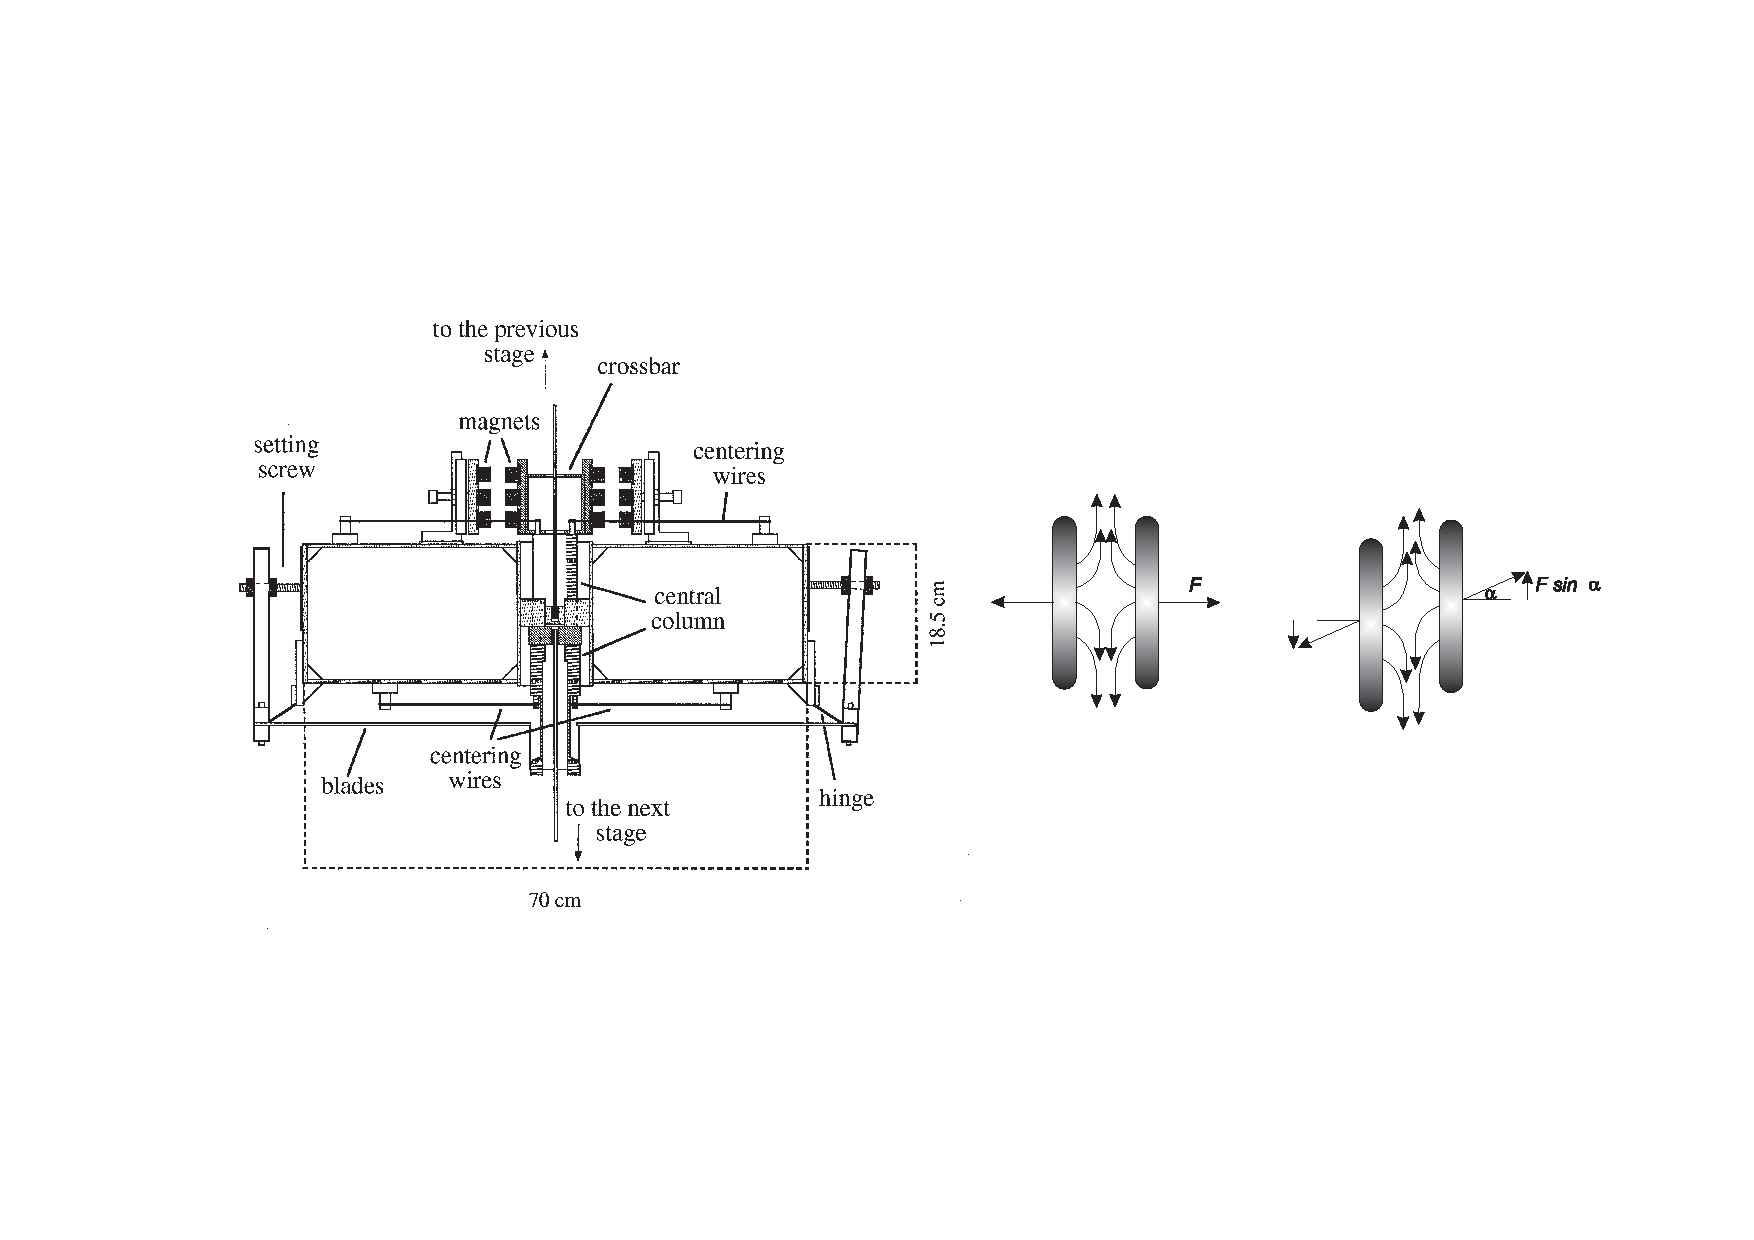
\includegraphics[width=17cm]{./Sec_Suspensions/Figures/SAfig2.pdf}
			\caption{The Virgo seismic filter: a technical drawing (\emph{left side}). The working principle of the magnetic anti-spring system accommodated on the seismic filter crossbar (\emph{right side}).}
\label{SAfig2}
	\end{center}
\end{figure}
%%

\subparagraph{The Seismic Filters}
In the Virgo \emph{Superattenuator} each pendulum mass has been replaced by a rigid metallic structure drum shaped acting as an oscillator in vertical direction too. A sequence of six mechanical filters is able to isolate the optical components from seismic noise in accordance with the working principle of a multistage pendulum (see Fig.~\ref{SAfig1}). A detailed description of the design and performance of a single filter can be found in reference~\cite{Beccaria1997}. A seismic filter is a rigid steel cylinder (70\,cm diameter, 18.5\,cm high for a total weight of about 100\,kg) suspended as close as possible to its centre of mass (see Fig.~\ref{SAfig2} left side). On the outer circumference of its body bottom part, a set of triangular cantilever spring blades is clamped. Each blade (3.5\,mm thick and 385.5\,mm long) is bent at a constant curvature radius and with different base width according to the load to be supported. A nominal load, ranging between 48\,kg and 96\,kg hung on the blade tip, forces it in flat and horizontal position. The blade tip is connected by a 1\,mm diameter wire to a central column, inserted through a hole in the centre of the filter body. Any movement of the central column, apart from the vertical direction, is prevented by two sets of four centreing wires accommodated on the top and on the bottom of the filter body.

A crossbar, bolted on the upper part of the central column, is used as a mechanical support for the magnetic anti-spring system described in the next sub-paragraph. The central column and the crossbar, connected to the blade spring, represent the moving part of the mechanical filter from which the load of the lower stages is suspended by a steel suspension wire. By connecting each filter to the next one, a chain of mechanical oscillators in vertical direction is obtained.

According to the previous description of our filtering system it is clear that the total load of the chain is suspended by the triangular steel blades. The base width of the triangle ranges from 180 to 110\,mm in accordance with the load to be supported. For the same reason the top filter is equipped with 12 blades while the last one needs only four blades.Once properly loaded the main vertical resonant frequency of each filter is about 1.5\,Hz. 

Maraging steel has been used in place of standard steel for blade construction in order to minimize micro-creep effects~\cite{Beccaria1998,Braccini2000} due to the high load applied. The same material has been used to machine the suspension wires with nail-head at both ends~\cite{Delapierre1997}. Since the suspended load decreases going from the top to the bottom of the chain, the wire and the nail-head diameters change along the chain in the ranges 4--1.85\,mm and 8--6\,mm, respectively. In this way it has been possible to confine the violin vibration mode within the high frequency band and to reduce its angular stiffness which determines the rotational frequency around the vertical axis. 

The two nail-heads of the wires connecting a filter on the chain to the previous and to the next one are screwed in the central part of its body at a relative distance of 5\,mm, very close to the filter centre of mass. As mentioned above, this guarantees a small return torque to rotations of the filter around the horizontal axis and thus a low tilt frequency.

\subparagraph{The magnetic anti-spring}
The suspension wire length of 1.15\,m in the Virgo \emph{Superattenuator} sets the pendulum resonant frequency of each stage at about 0.5\,Hz. In the vertical direction the stiffness of the triangular blade springs fixes the natural resonant frequency at about 1.5\,Hz. In order to reduce the vertical stiffness of the blades, and then to confine the main vertical resonant frequency of each filter below the pendulum one, a system of magnetic anti-springs \cite{Beccaria1997,Braccini1993} has been adopted (see Fig.~\ref{SAfig2} left side). It consists of two sets of permanent magnets (the first assembled on the crossbar and the second one on the filter body), facing each other with opposite horizontal magnetic moment (namely in a repulsive configuration). In this way the two matrices screwed on the crossbar are forced to move in vertical direction only. 

When the magnets are perfectly faced the repulsive force has a null vertical component, but as soon as a matrix is moved in the vertical direction, a vertical component of the magnetic force appears. Considering a small relative displacement ($\Delta{y}$), compared with the distance ($d$) between two matrices of magnets and with their transverse dimension, the vertical component of the repulsive force ($F_y$) is proportional to $\Delta{y}$:

\beq
F_{y}\approx F_{0}\cdot (\Delta y/d)
\label{mag}
\eeq

where $F_0$ is the modulus of the repulsive force (see its working principle in Fig.~\ref{SAfig2} right side). Such device is equivalent to a vertical spring with a negative elastic constant (anti-spring) whose modulus is $F_0/d$. Thus, its rest position is that of  the two couple of matrices perfectly faced. On a seismic filter the magnetic anti-springs act on the crossbar in parallel with the blade springs, so that the vertical modes frequency of the chain are confined below the highest frequency of the horizontal ones. 
The advantages of this system are the vacuum compatibility and the contact-less
action performed on the filter, for this reasons it represents the reference solution for the third generation detector.

An evolution of the Virgo mechanical filter to be used as vertical seismic noise  
suppression system, is the Geometric Anti Spring (GAS) filter described in the appendix \ref{sec:Gas_spring}. It was proposed  by R. De Salvo et al.~\cite{cella} few years ago and it has been tested in TAMA. 
The GAS filter is used as seismic isolation system for the 10 m 
long interferometer at AEI Hannover and the same technology is developed by the NIKHEF group for the optical bench of the light injection in the interferometer for Advanced Virgo.


\subparagraph{The Steering Filter} \label{steeringF}

The last mechanical filter of the Virgo seismic attenuation chain is the Steering Filter~\cite{Ballardin2001}. It has been designed to suspend and orientate the payload, a multi-body mechanical system whose core is a test-mas of the gravitational-wave detector, by means of forces exerted within the suspension. The payload plays a crucial role in the overall dynamics 
of the system and its presence has been included in all the projections shown in this section of the report, assuming a basic design similar to that one actually developed for Virgo (Fig.~\ref{SAfig1}). However a dedicated section~\ref{sec:last_stage} will be devoted to the issues related to this 
system provided its crucial role in dealing with test-masses as mirrors of the interferometer. In the Virgo experimental apparatus the steering filter has been equipped with four Aluminium legs (about 900\,mm long and 250\,mm in diameter) bolted on the filter body bottom part. These legs are the mechanical support of the coils mounted in front of the permanent magnets screwed on the marionette wings and used to control the payload position.

In addition the Steering Filter is equipped with different vacuum compatible stepping motors. Two of them are dedicated to the filter alignment around its vertical axis. The first one is accommodated on top of the filter body and it is used to move the filter and the payload with respect to the upper part of the \emph{Superattenuator} while the second one is mounted at the bottom of it to change the relative position of the filter with respect to the payload. This last one is used to optimize the coil-magnet distance for the actuation on payload. A second pair of vacuum compatible stepping motors completes 
a set of remote controlled devices mounted on this mechanical filter. By moving some small masses attached to a mechanical trolley on top of the filter body, a fine adjustment of the tilt (rotations around the two horizontal axes) can be performed. 


\paragraph{c) Seismic isolation measurements with the Superattenuator (SA)}

The attenuation performance of the \emph{Superattenuator} has been measured by using the Virgo interferometer. In particular, a direct measurement of the mechanical transfer function has been obtained exciting with sinusoidal forces the top stage of  the mechanical filter chain. The measurement consists in detecting the presence of a spectral line with the same excitation frequency at the level of the mirror, i.e.\ at the interferometer dark port. The ratio between the linear spectral density at the excitation frequency of the mirror and that one of the top stage displacement (measured by means of the accelerometers) provides a measurement of the \emph{Superattenuator} mechanical transfer function magnitude. When the line is not detected at the level of the interferometer, only an experimental upper limit of the transfer function amplitude can be given. We remind that the linear spectral density of the noise floor of the top stage sensors or of the interferometer dark port, does not depend on the time length of the measurement while the amplitude of a spectral line increases with square root of the time interval. The longer is the integration time, the higher is the capability to distinguish a spectral line from the interferometer noise floor. Moreover, in those measurements where the peak is not distinguished at the level of the mirror, the upper limit of the transfer function, given by the ratio between the noise spectral floor and the top stage peak at the excitation frequency, improves (i.e.\ becomes smaller) increasing the integration time. In this case, the linear spectral density of the excitation line (denominator) becomes larger, while the interferometer noise floor (numerator) does not change.

A campaign of measurements has been performed exciting the suspension top stage both in horizontal laser beam direction and in vertical direction. The excitation is applied to the suspension point through the coil-magnet actuators used in the Inertial Damping of the chain resonance modes. The experimental results have been compared with the requirements of the future generation detectors (as reported also in Fig.~\ref{FigSusp3}) and plotted in Fig.~\ref{FigSusp5}.

\begin{figure}[t]
	\begin{center}
		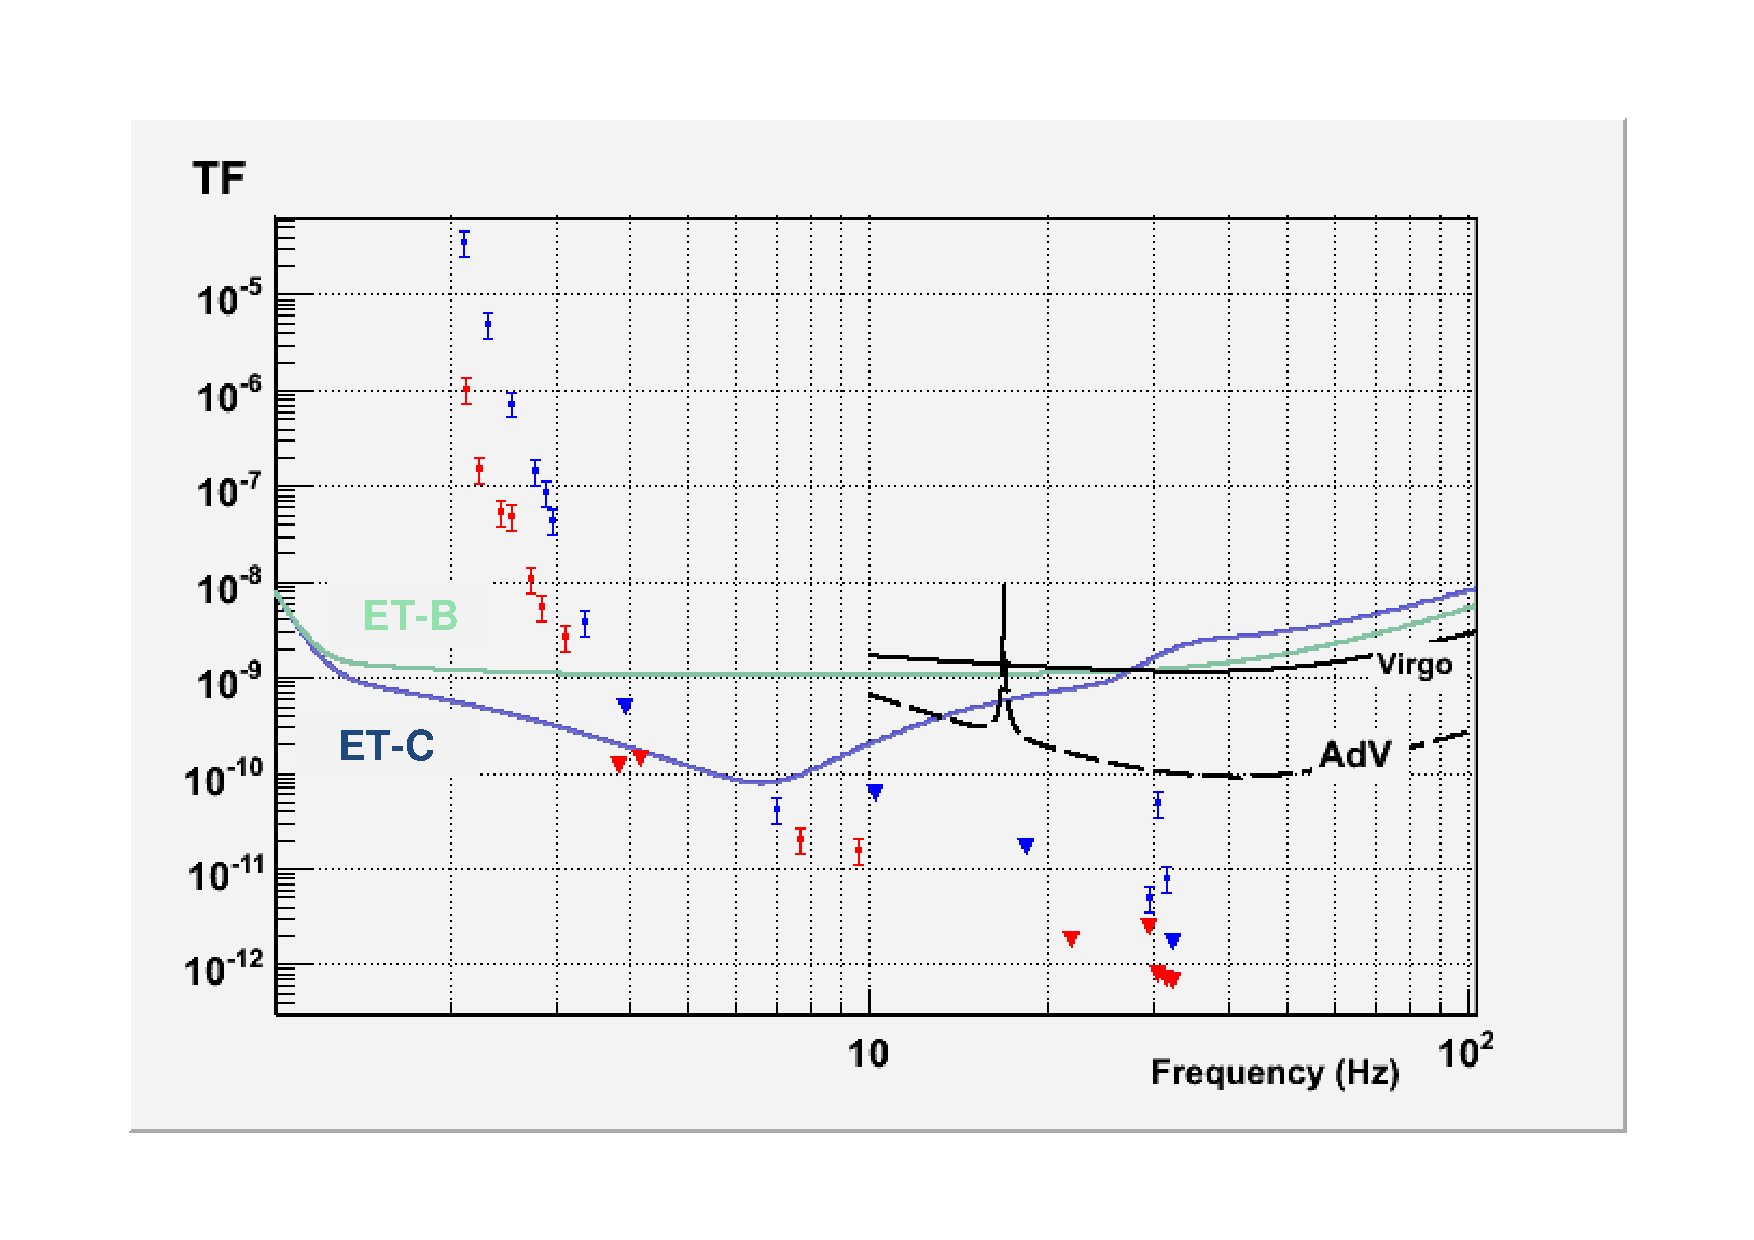
\includegraphics[width=0.9\textwidth]{./Sec_Suspensions/Figures/Fig5.pdf}
			\caption{The measurement of the transfer functions at different frequencies. In red are reported the measurements where a vertical excitation of the top stage is applied. In blue are the measurements with the excitation in horizontal direction. The upper limits are indicated by triangles, while the direct measurements (when a signal is detected at the level of the mirror) are indicated with the bars. For the discussion of the error bars see reference~\cite{Collaboration2010}.}
\label{FigSusp5}
	\end{center}
\end{figure}

Above 3 Hz all the measured transfer functions (upper limits or direct measurements) turn out to be within the requirements of Einstein Telescope. Changes to the \emph{Superattenuator} structure (such as a length extension of the filter chain) will be needed in Einstein Telescope only in the case the detection threshold frequency will be moved below 3 Hz. In reference \cite{Ballardin2001}, where a stage by stage (indirect) measurement of the \emph{Superattenuator} total transfer function (valid at any frequency) has been provided (and compared with simulation), a very steep behavior around 3 Hz is well visible. Considering this as a reference result, it is clear that even changing by a couple of orders of magnitude the input seismic noise as well as the attenuation requirements, the crossing frequency between the transfer function and the requirement curve should remain around 3 Hz. 

In addition, around 30 Hz and in the 7-9 Hz region, our measurements put in evidence some peaks above the interferometer noise floor while excitation is applied on the top stage. This is an indication of noise transmission a couple of orders of magnitude larger than expected from simulation and indirect measurements (stage by stage). However, also in these cases, the transfer function has been measured to not exceed the detector requirements. Other mechanisms could cause the detected tiny motion of the mirror by-passing the extremely high mechanical attenuation, as discussed in \cite{Collaboration2010, Braccini2010March1-3}. The extension of the multistage pendulum length, linked to the need of moving down below 2 Hz the cross-over between the horizontal seismic noise and the antenna sensitivity (see next section), is welcome for a better separation of the top-stage control and the optical payload control preventing cross-talks.

It is important to stress that, during our measurements campaign, the pre-isolator stage (described above) has been excluded from the transfer functions measurements. So that an additional attenuation factor, of the order of 20--40\,dB, has to be considered as safety margin. With this additional attenuation factor, one can conclude that the cross-over for the Einstein Telescope requirements is expected to be around 2.8\,Hz by using the present \emph{Superattenuator} scheme. The cross-over is dominated by horizontal seismic noise.


\paragraph{d) SA modifications for Low Frequency ET}

In order to extend the detection bandwidth of the Einstein Telescope in the low-frequency region starting from a couple of Hz, a better seismic attenuation in the ultra-low frequency range is needed. To this purpose a detailed simulation campaign devoted to this design study has been performed. The SA dynamics in the low frequency range, where the inner normal modes of the mechanical filter chain are confined, can be well simulated by using the electro-magnetic equivalent circuit (a series of oscillators). 
A maximization algorithm, called \emph{Simplex}~\cite{Different2008_SecondEdition}, based on the possibility to change the masses and the mechanical filter chain lengths, has been developed. It searches for a maximum attenuation performance at a fixed frequency that, in our case, was 2\,Hz.  Since the transfer function has a smooth shape, it turns out that to get a higher attenuation at 2\,Hz, we should have a lower  "cross-over frequency" with the requirements curves (see Fig.~\ref{Par4Fig1}). As showed in the direct measurement performed with the Virgo interferometer (see section 4.1.1.c), the cross-over between seismic noise at the mirror level and the requirements is dominated by the residual horizontal seismic vibrations. For this reason to move the cross-over at lower frequency, we need to improve  the attenuation performance of the horizontal seismic vibration in the low frequency range.
%
\begin{figure}[t]
	\begin{center}
		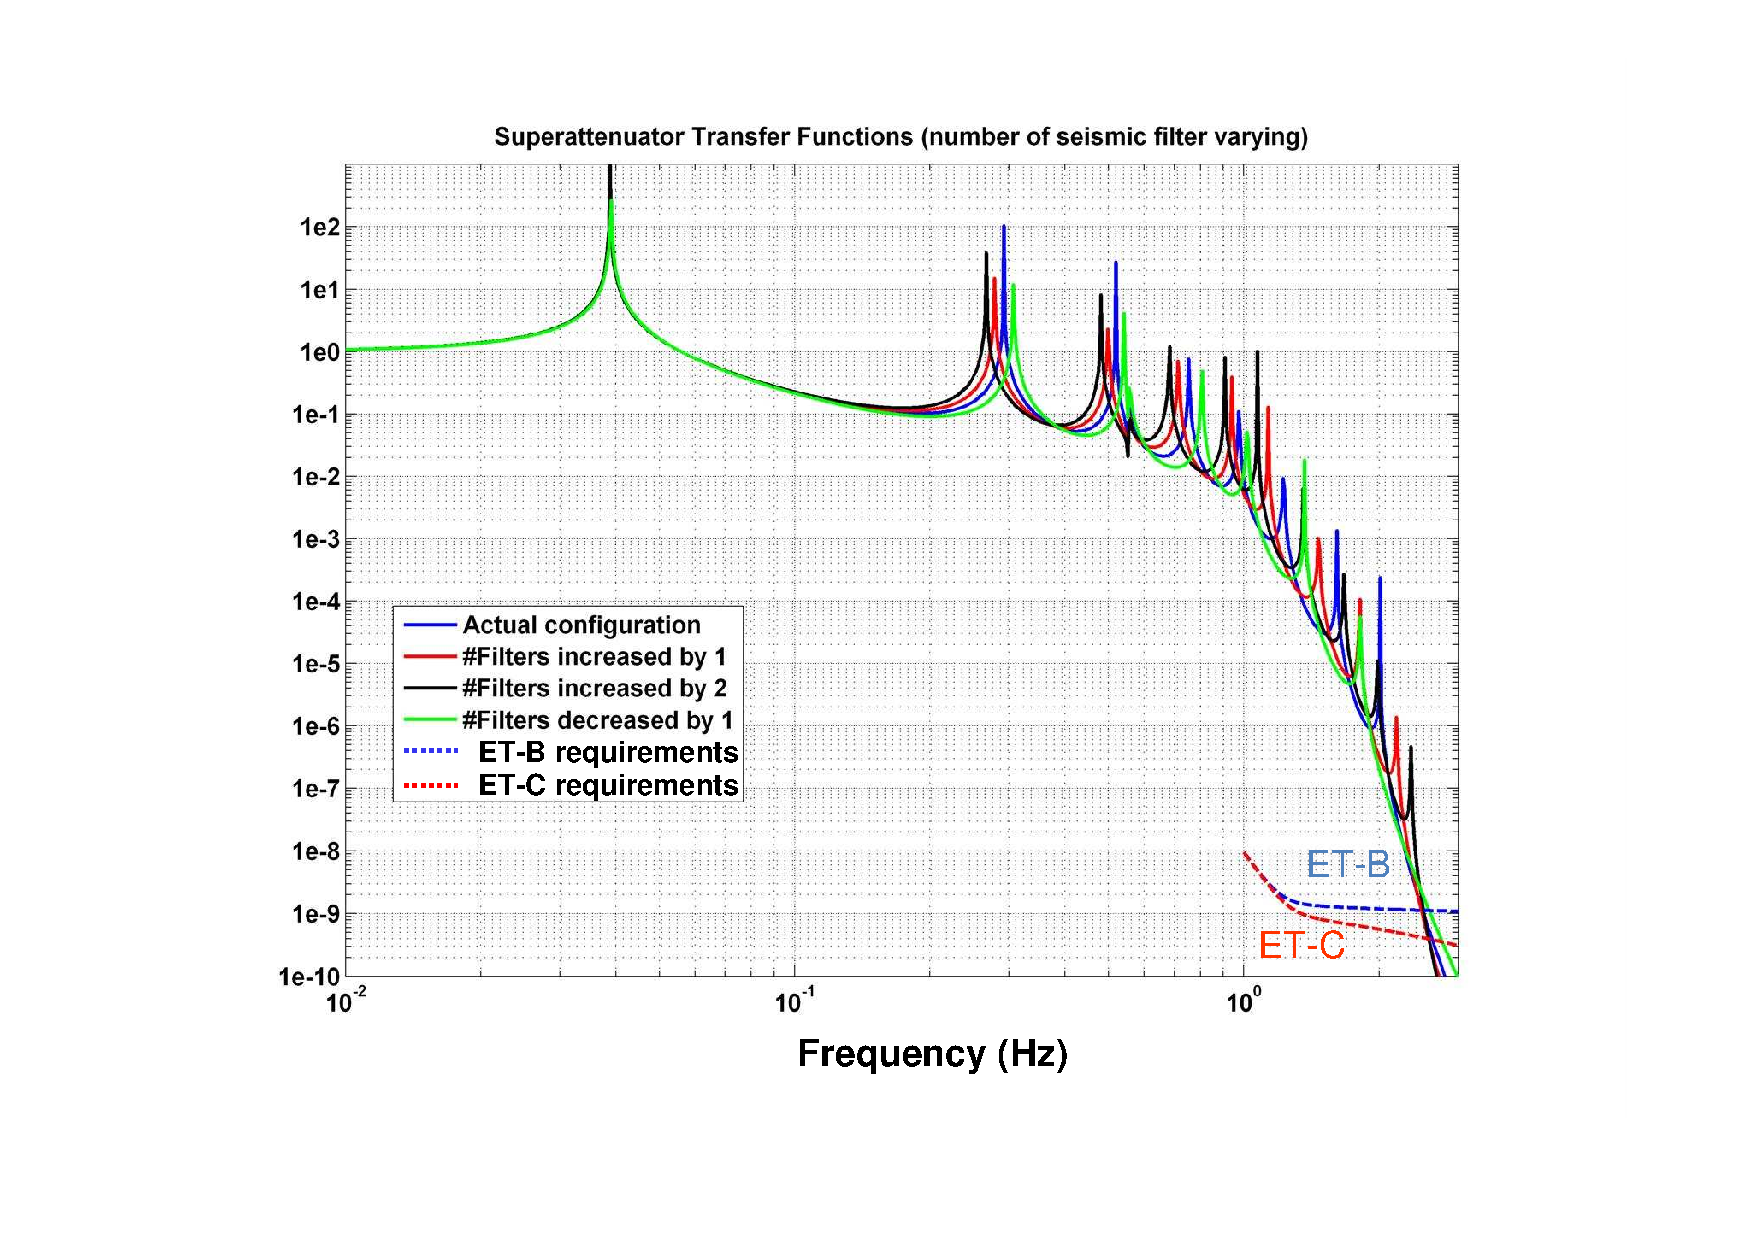
\includegraphics[width=0.9\textwidth]{./Sec_Suspensions/Figures/Par4-Fig1.pdf}
			\caption{Simulation results of the SA horizontal transfer function with the present chain length (9 m). Changing the number of (``equal-spaced'') filters the resulting horizontal transfer function is compared with the ET requirements (for High Frequency---\emph{ET-B}---and low frequency or ``xylophone'' configuration---\emph{ET-C}). Adding or removing filters along the chain length do not have remarkable role in the positioning of the cross-over frequency with the requirements.}
\label{Par4Fig1}
	\end{center}
\end{figure}
%
An important preliminary conclusion of our design study is that, fixing the length and the number of mechanical filters, the optimal configuration (i.e.\ that one minimizing the cross-over frequency or maximizing the attenuation performance at 2\,Hz) is that one where the filters are separated along the chain by the same distance. This "equal-spaced" configuration represents the optimal one even because the vertical transfer function is not influenced by the filter positioning along the chain. Moreover it has been proved that increasing\,/\,decreasing the number of filters or changing their masses do not play a fundamental role in determining the cross-over frequency between the horizontal transfer function and the requirements. The results obtained are plotted in Fig.~\ref{Par4Fig1} and Fig.~\ref{Par4Fig2} while in the corresponding captions complementary information is available.  
%
\begin{figure}[t]
	\begin{center}
		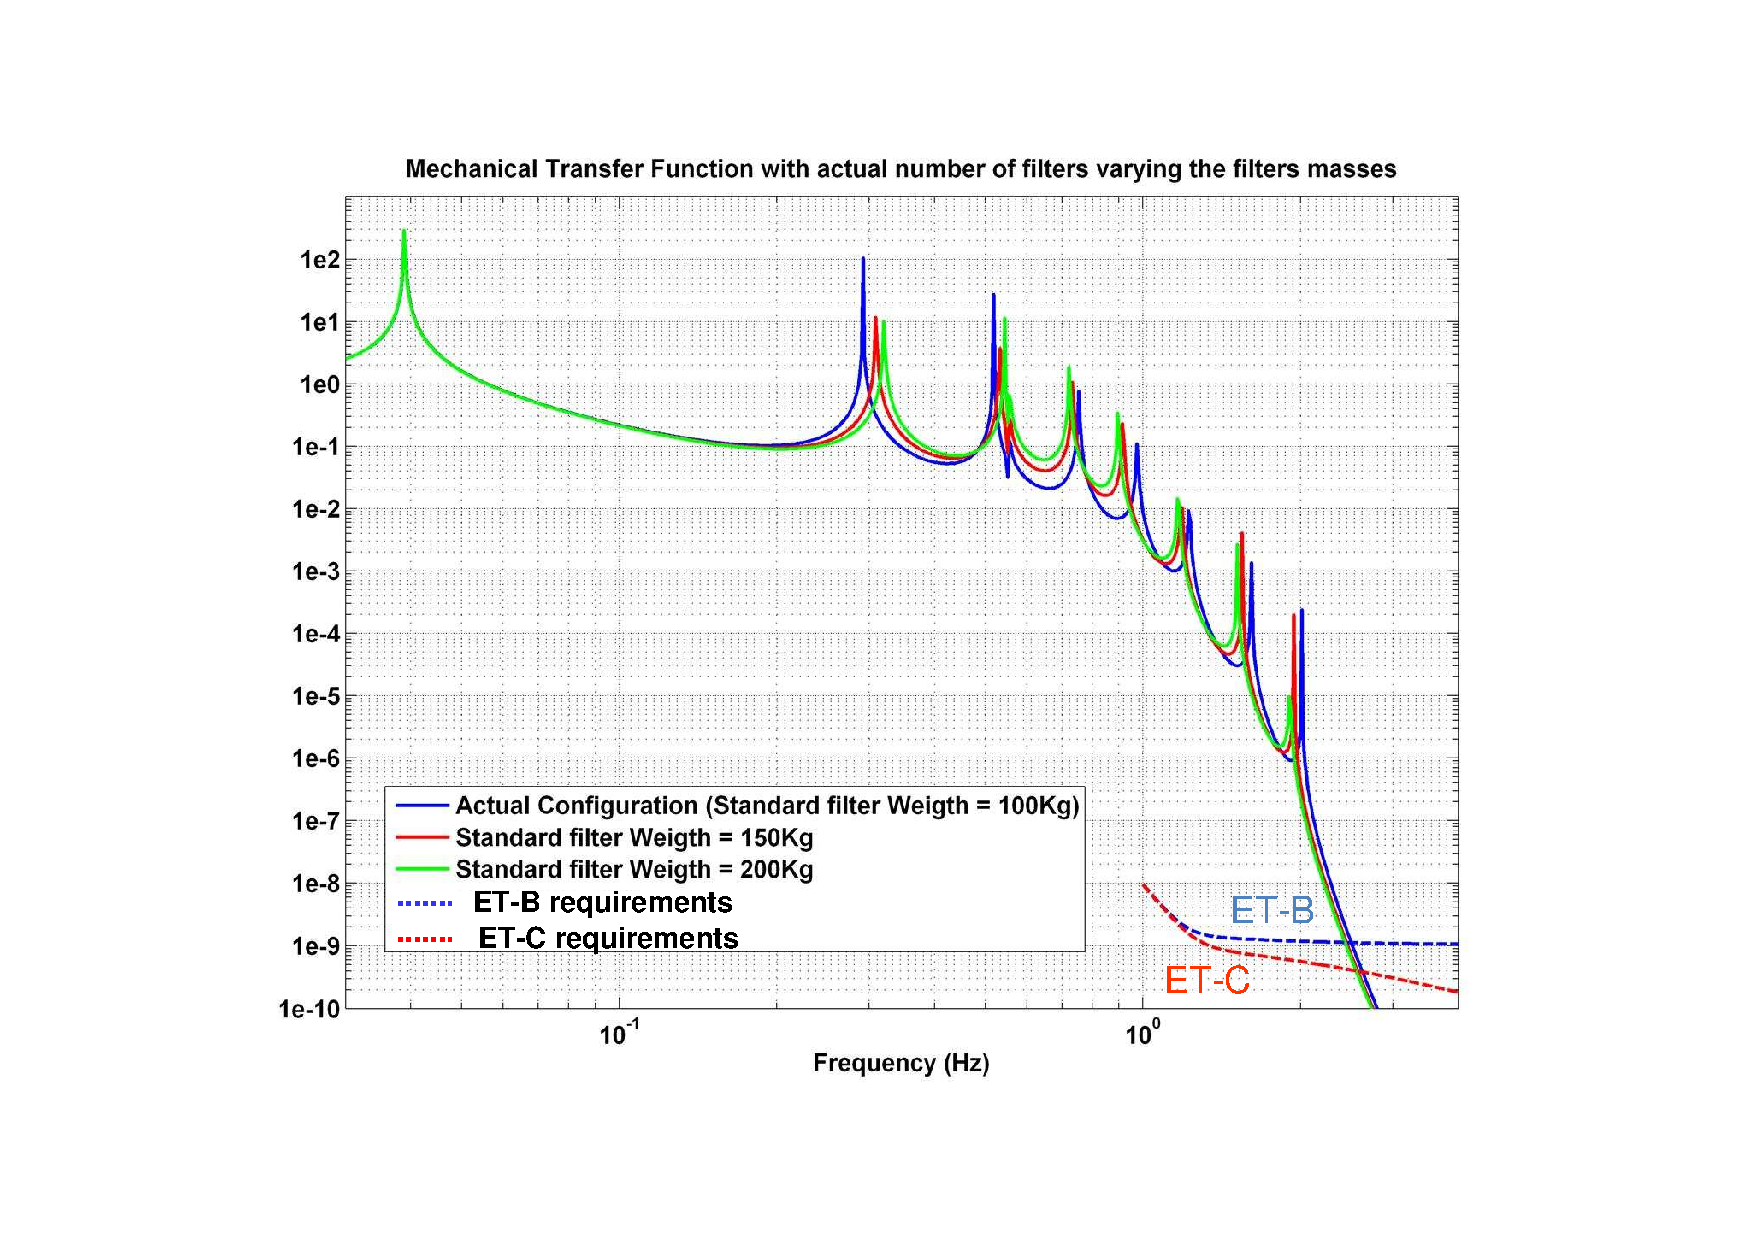
\includegraphics[width=0.9\textwidth]{./Sec_Suspensions/Figures/Par4-Fig2.pdf}
			\caption{The horizontal transfer function of the present \emph{SA} (6 filters weighting 100\,kg each one for a total length of about 9\,m) is compared with the same transfer function changing the mass of each filter (150\,kg and 200\,kg). Also in this case the cross-over frequency with the ET requirements is not remarkably affected by the change of the filter mass.}
\label{Par4Fig2}
	\end{center}
\end{figure}
%
\begin{figure}[t]
	\begin{center}
		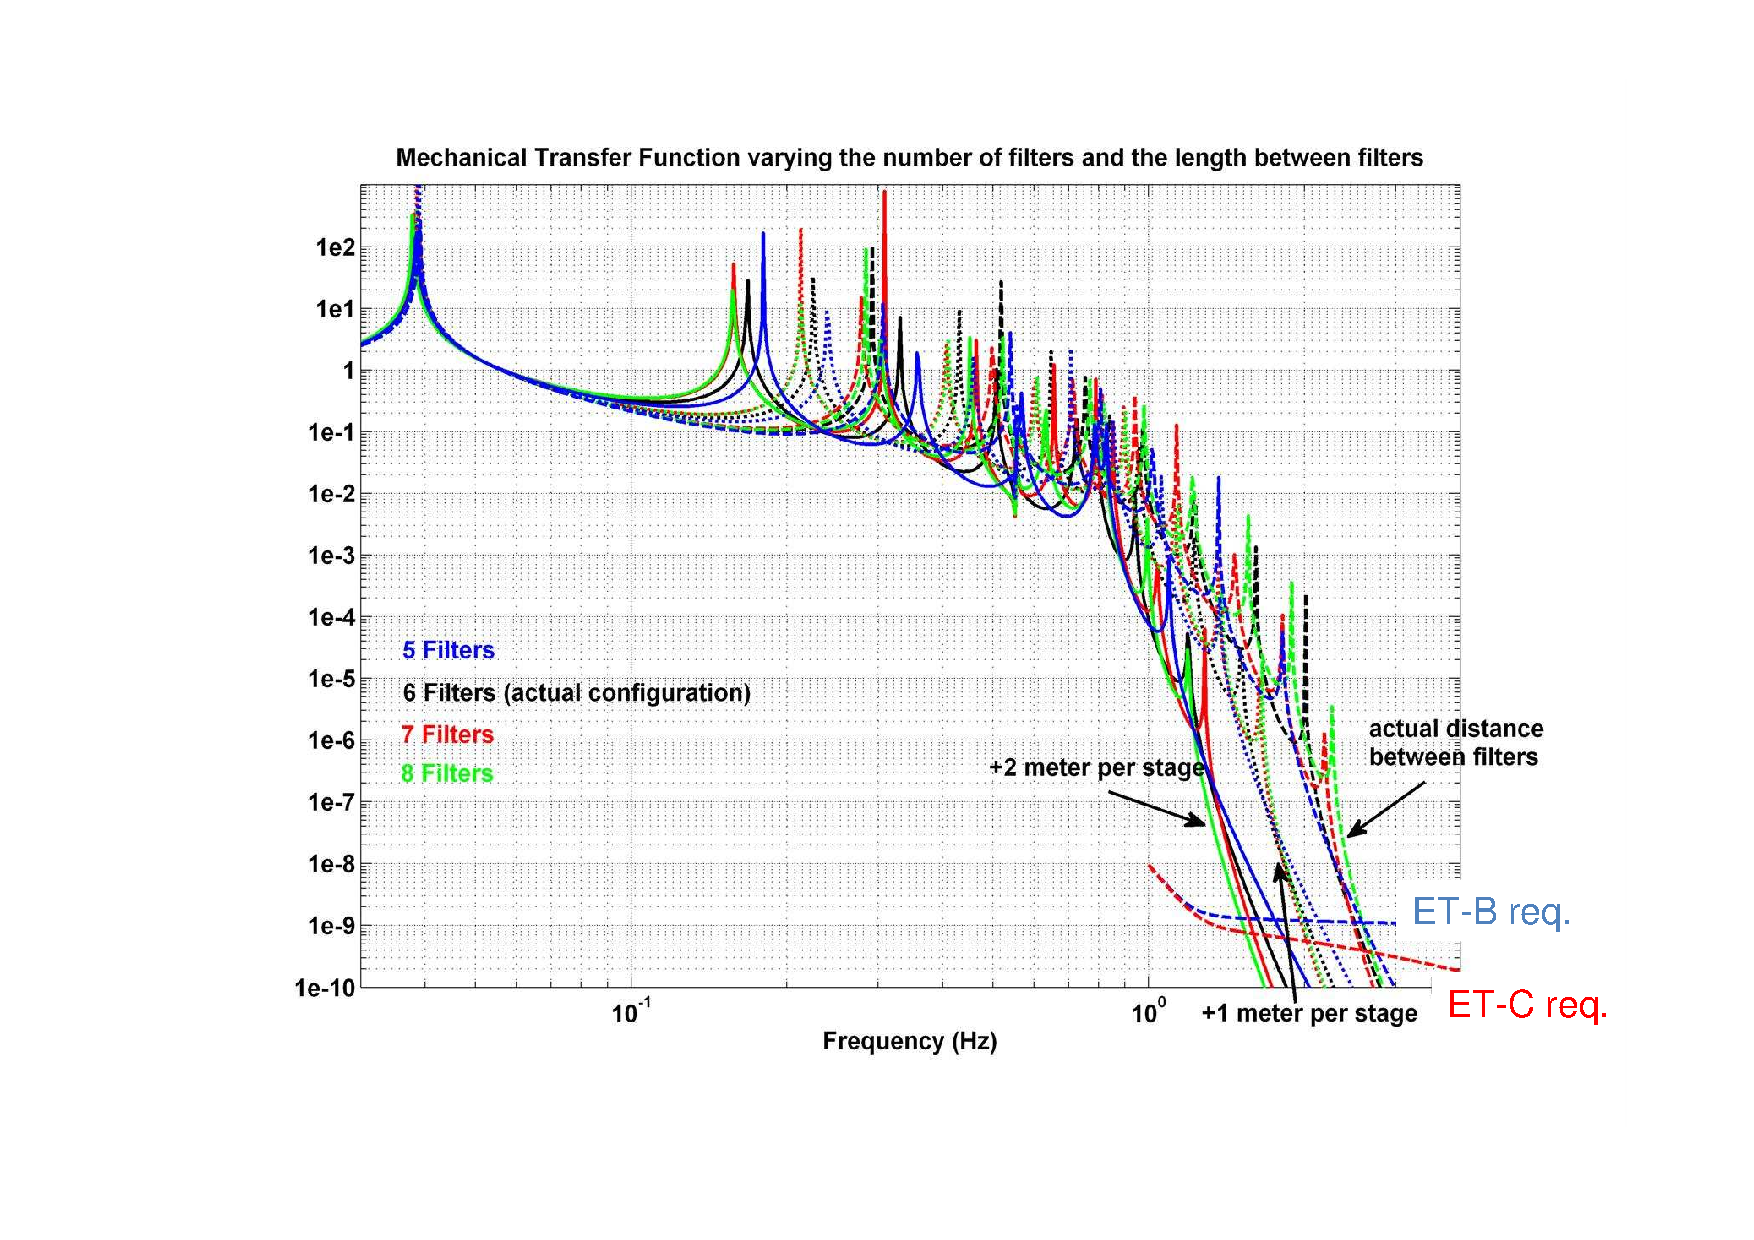
\includegraphics[width=0.9\textwidth]{./Sec_Suspensions/Figures/Par4-Fig3.pdf}
			\caption{Simulation results for different configurations. The horizontal transfer function of the \emph{SA} is plotted changing the number of filters and keeping fixed their relative distances ("equal-spaced" geometry) along the chain (changing, as a consequence, the full length of the SA).}
\label{Par4Fig3}
	\end{center}
\end{figure}
%
The only way to move in the low frequency region the cross-over frequency extending the Einstein Telescope bandwidth below 3 Hz, is to increase the SA chain total length. The simulation results for different configurations can be found in figure~\ref{Par4Fig3} and described in~\cite{Braccini2010March1-3}, while the best solution seems to be represented by a SA with 6 filters and a total length of 17\,m (identical the Virgo configuration, where 5 mechanical filters suspended from an horizontal pre-isolator stage plus the marionette are assembled forming a filter chain about 9\,m long). As shown in Fig.~\ref{Par4Fig4}, with this solution the cross-over frequency has been placed around 1.7--1.8\,Hz, that is considered enough for our purpose. Indeed, Newtonian noise and other technical noise are assumed to prevent an effective detection above a couple of Hz.
%
\begin{figure}[t]
	\begin{center}
		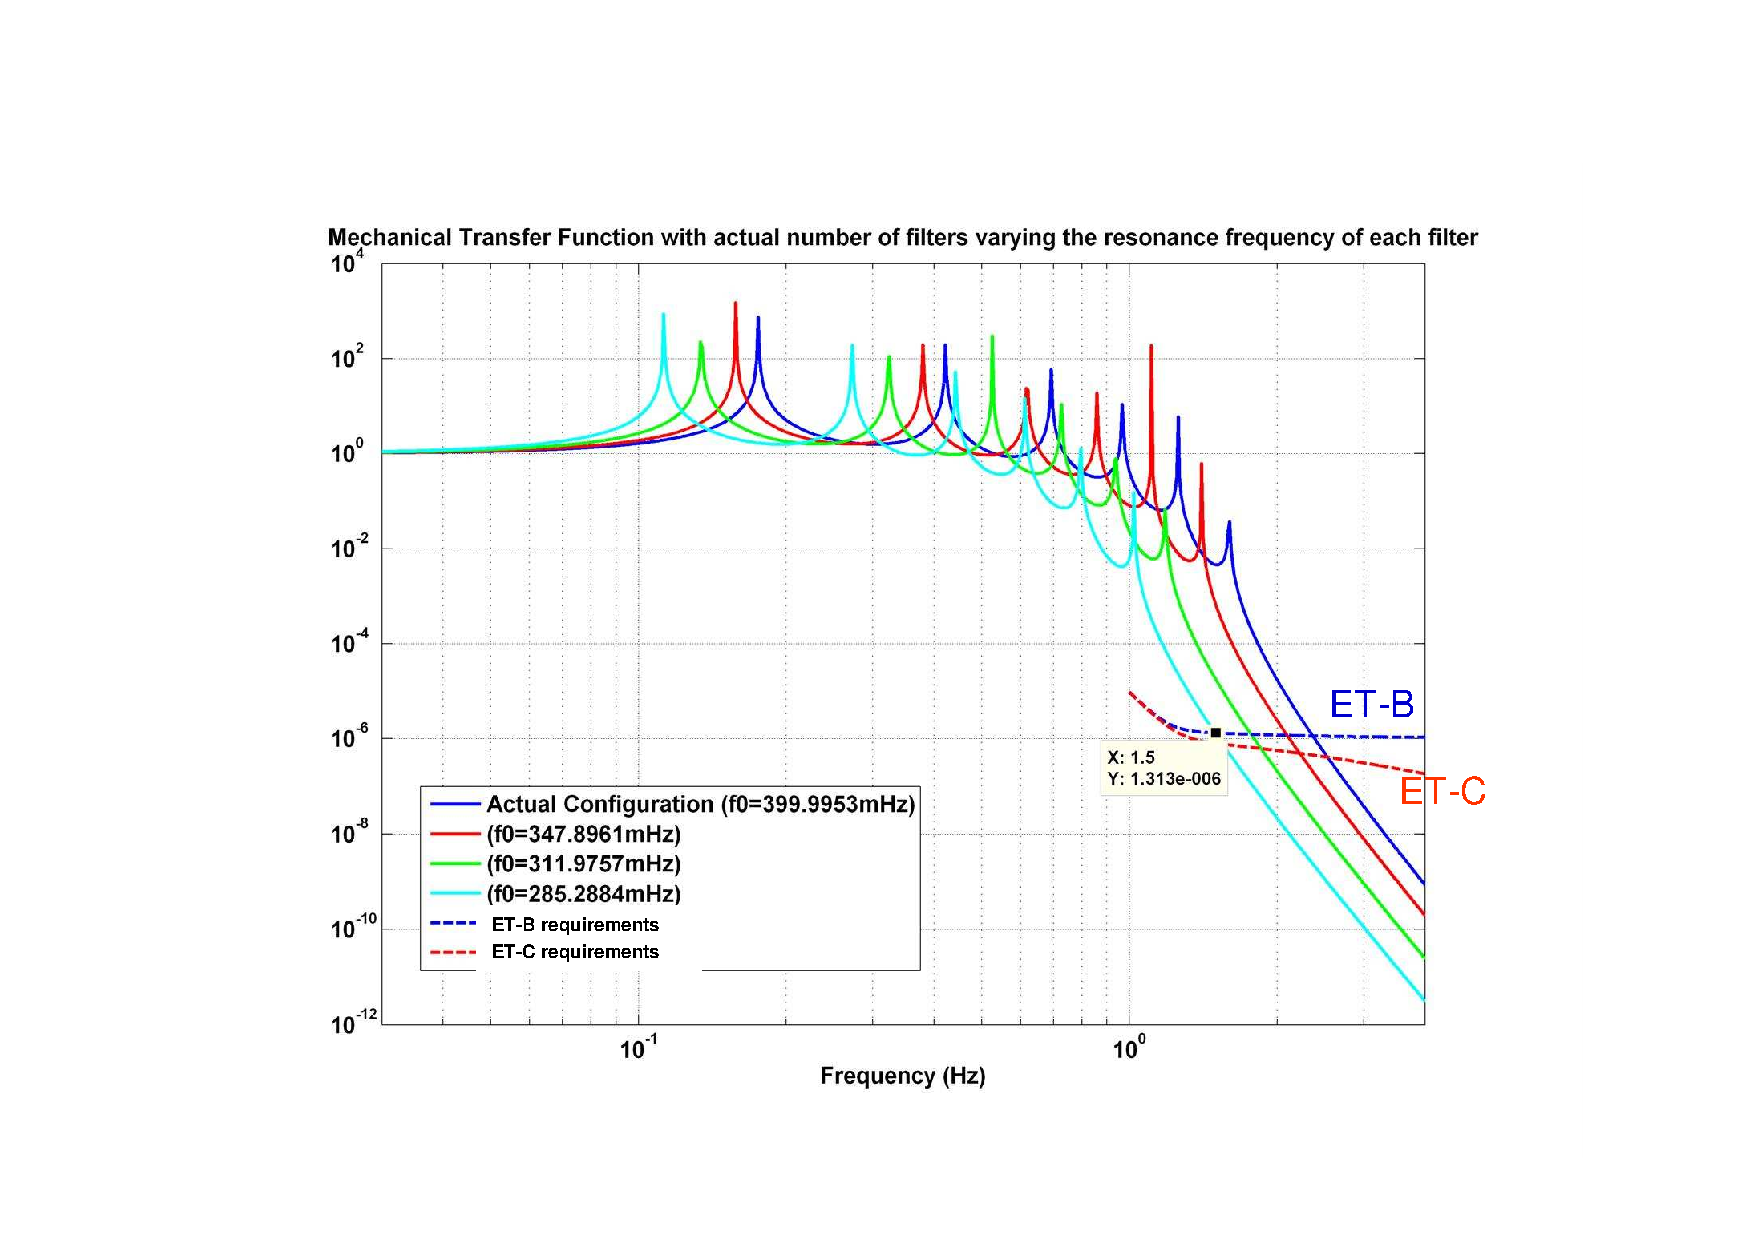
\includegraphics[width=0.9\textwidth]{./Sec_Suspensions/Figures/Par4-Fig5.pdf}
			\caption{Vertical Transfer Function of the SA considering the six stages (as it is now, i.e.\ with the pre-isolator or ``Filter Zero'' plus other five mechanical filters). The different curves have been obtained changing the filter vertical resonant frequency. With filters working around 300\,mHz it is possible to move the cross-over below 2\,Hz.}
\label{Par4Fig5}
	\end{center}
\end{figure}
%
With this configuration, the vertical cut-off frequency of the whole system is set below 1.8\,Hz by tuning each mechanical filter having the main vertical frequency around 300\,mHz (see Fig.~\ref{Par4Fig5}). The corresponding vertical transfer function is plotted in Fig.~\ref{Par4Fig4}. Since the residual seismic noise along the vertical direction, at the level of the mirror, is expected to limit the Einstein Telescope sensitivity again around 1.7--1.8\,Hz, a coupling factor of $10^{-3}$ has been considered. This is due to the fact that the Earth curvature makes plumb lines at a 10\,km distance not parallel each other. At least one mirror has to be inclined with respect to the local plumb line performing the alignment of the cavities. This transmits the residual vertical mirror motion along the beam with the mentioned coupling factor ($10^{-3}$).
%
\begin{figure}[t]
	\begin{center}
		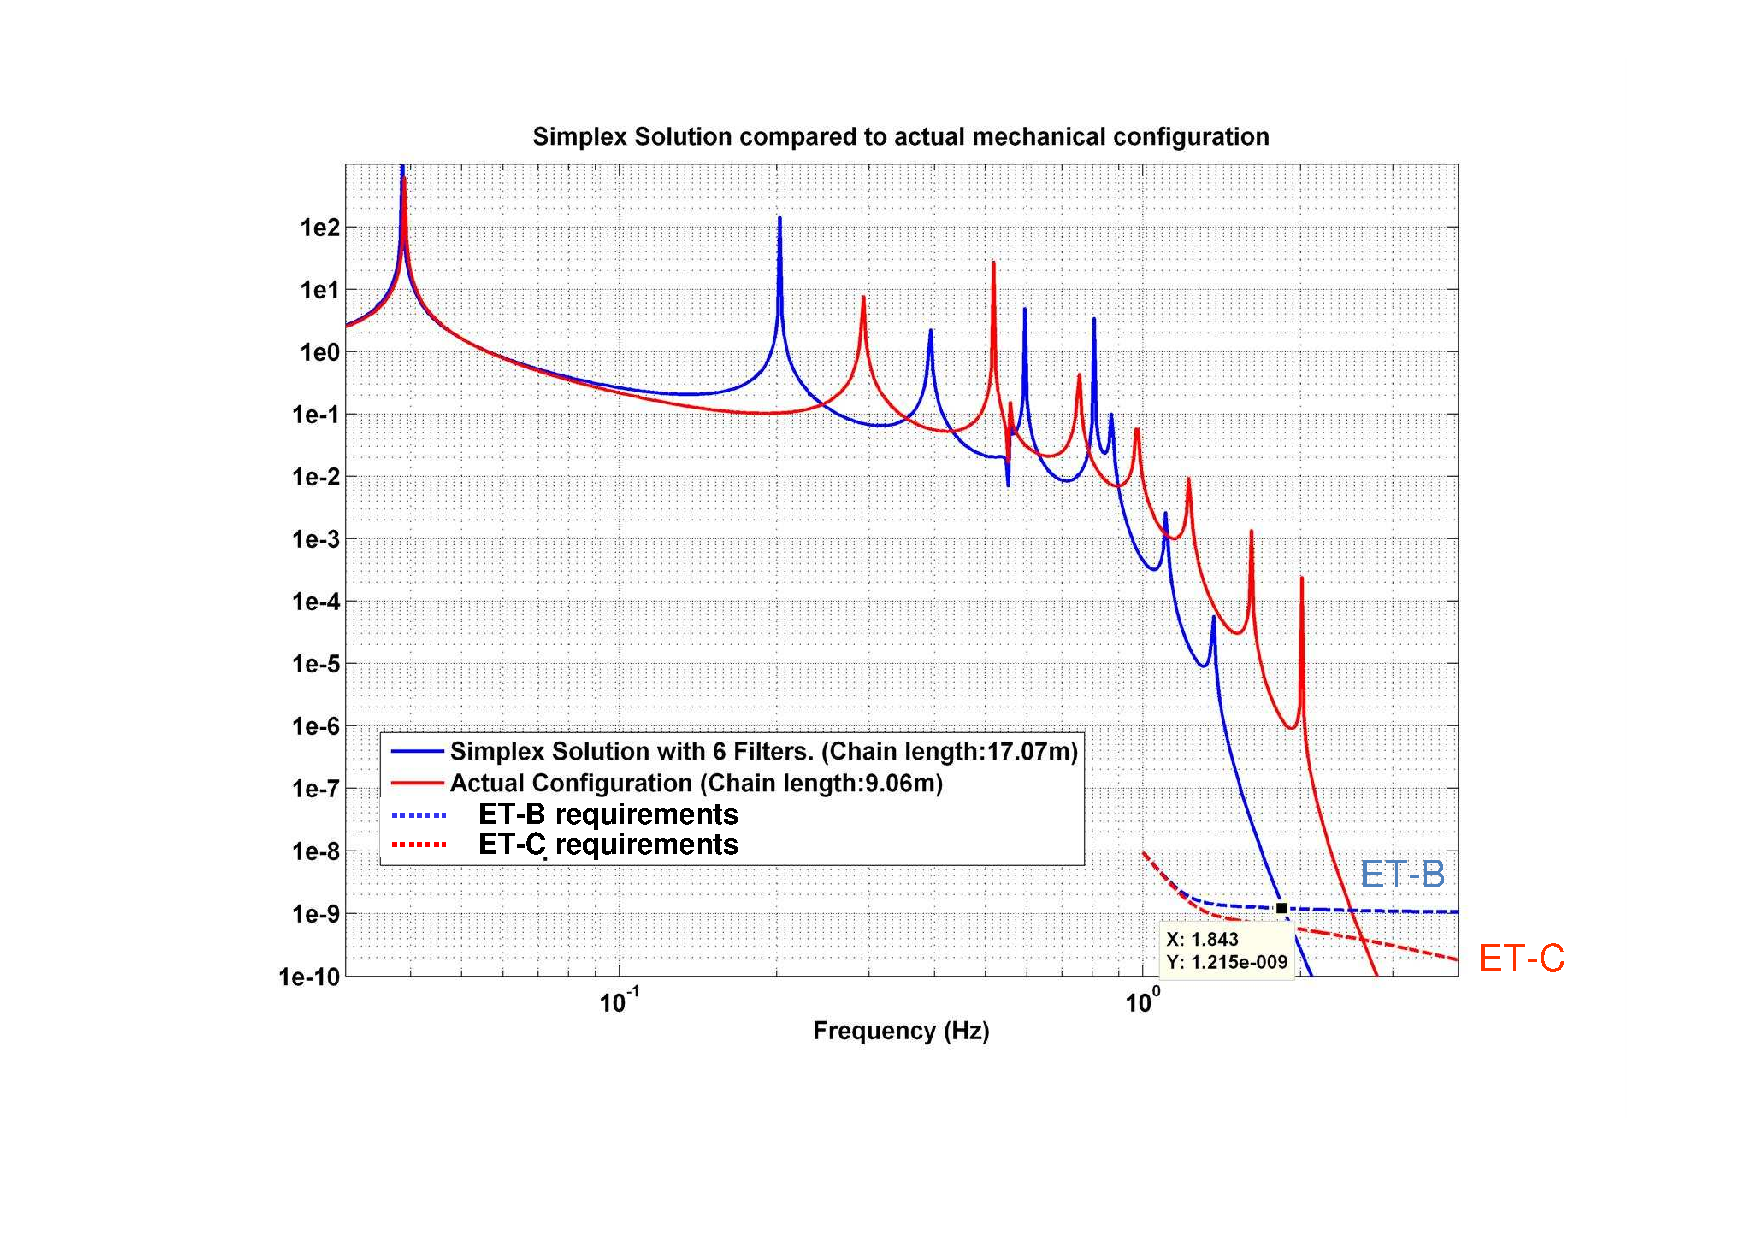
\includegraphics[width=0.9\textwidth]{./Sec_Suspensions/Figures/Par4-Fig4.pdf}
			\caption{The proposed reference solution for the $SA$ configuration of the Einstein Telescope. Other slightly different configurations are discussed in \cite{Braccini2010March1-3}.}
\label{Par4Fig4}
	\end{center}
\end{figure}
%
Since years in Virgo many mechanical filters with a cut-off frequency of around $300$ $mHz$ \emph{Superattenuators} are  in operation  with an excellent stability. By using the Virgo interferometer data, it has been observed that the long-term change of the chain main resonant frequencies induced by the temperature variation under vacuum are 
well inside the line-width of the chain vertical resonances. No effect on the interferometer control is due to this potential disturbance. Moreover, even if the temperature variations induce a motion of the suspension chain and then a slow vertical displacement ({\it {breath}}) of the mirror (a few $mm$ per $^{\circ}C$ is the measured 
value for the Virgo \emph{Superattenuator}), this effect is well within the specifications of any interferometer (vacuum tank provides an excellent temperature stability - fraction of $^{\circ}C$ peak to peak).
The standard SA, presently in operation on the Virgo interferometer, is already well inside the third generation specifications from this point of view too.

In addition, it is important to remind that the requirements in the tens of Hz range are less stringent in Einstein Telescope than in Advanced Virgo (see section 4.1.1.a) and thus, fixing to six (a choice lead by the reduction of the cross-over frequency) the number of filters, a better attenuation performance in the high frequency range is not necessary anymore since the safety margin is large enough in Advanced Virgo and even larger in an underground environment. In conclusion, a SA $17$ $m$ high with 6 magnetic anti-spring filters ("equal-spaced" configuration) tuned with a vertical cut-off frequency around 300 $mHz$, represents the reference solution for the Einstein Telescope. 

In the Appendix \ref{sec:LIGO_filters} we briefly describe the Advanced LIGO  approach to suppress seismic noise. It includes a large two-stages platform  fully active controlled, that, in principle, could improve the compactness of the  ET-LF chain. However a dedicated R\&D study is required for assessing the technical feasibility of this approach in the  ET-LF case.

\paragraph{e) Noise from SA mechanical micro-glitches}

The dislocation motion in the elastic elements of the anti-seismic filter under stress follow a ``self-organized criticality dynamics'' ~\cite{Marchesoni1994}  causing a mechanical noise force along the vertical direction. This force due to micro-glitches exhibits an ``$1/f$-spectrum'', and it is sometime called ``creep noise''. This noise mechanism could affect the interferometer sensitivity. For this reason the Virgo interferometer has been used to set upper limits on the noise floor induced by this spurious mechanism.
\begin{figure}[t]
	\begin{center}
		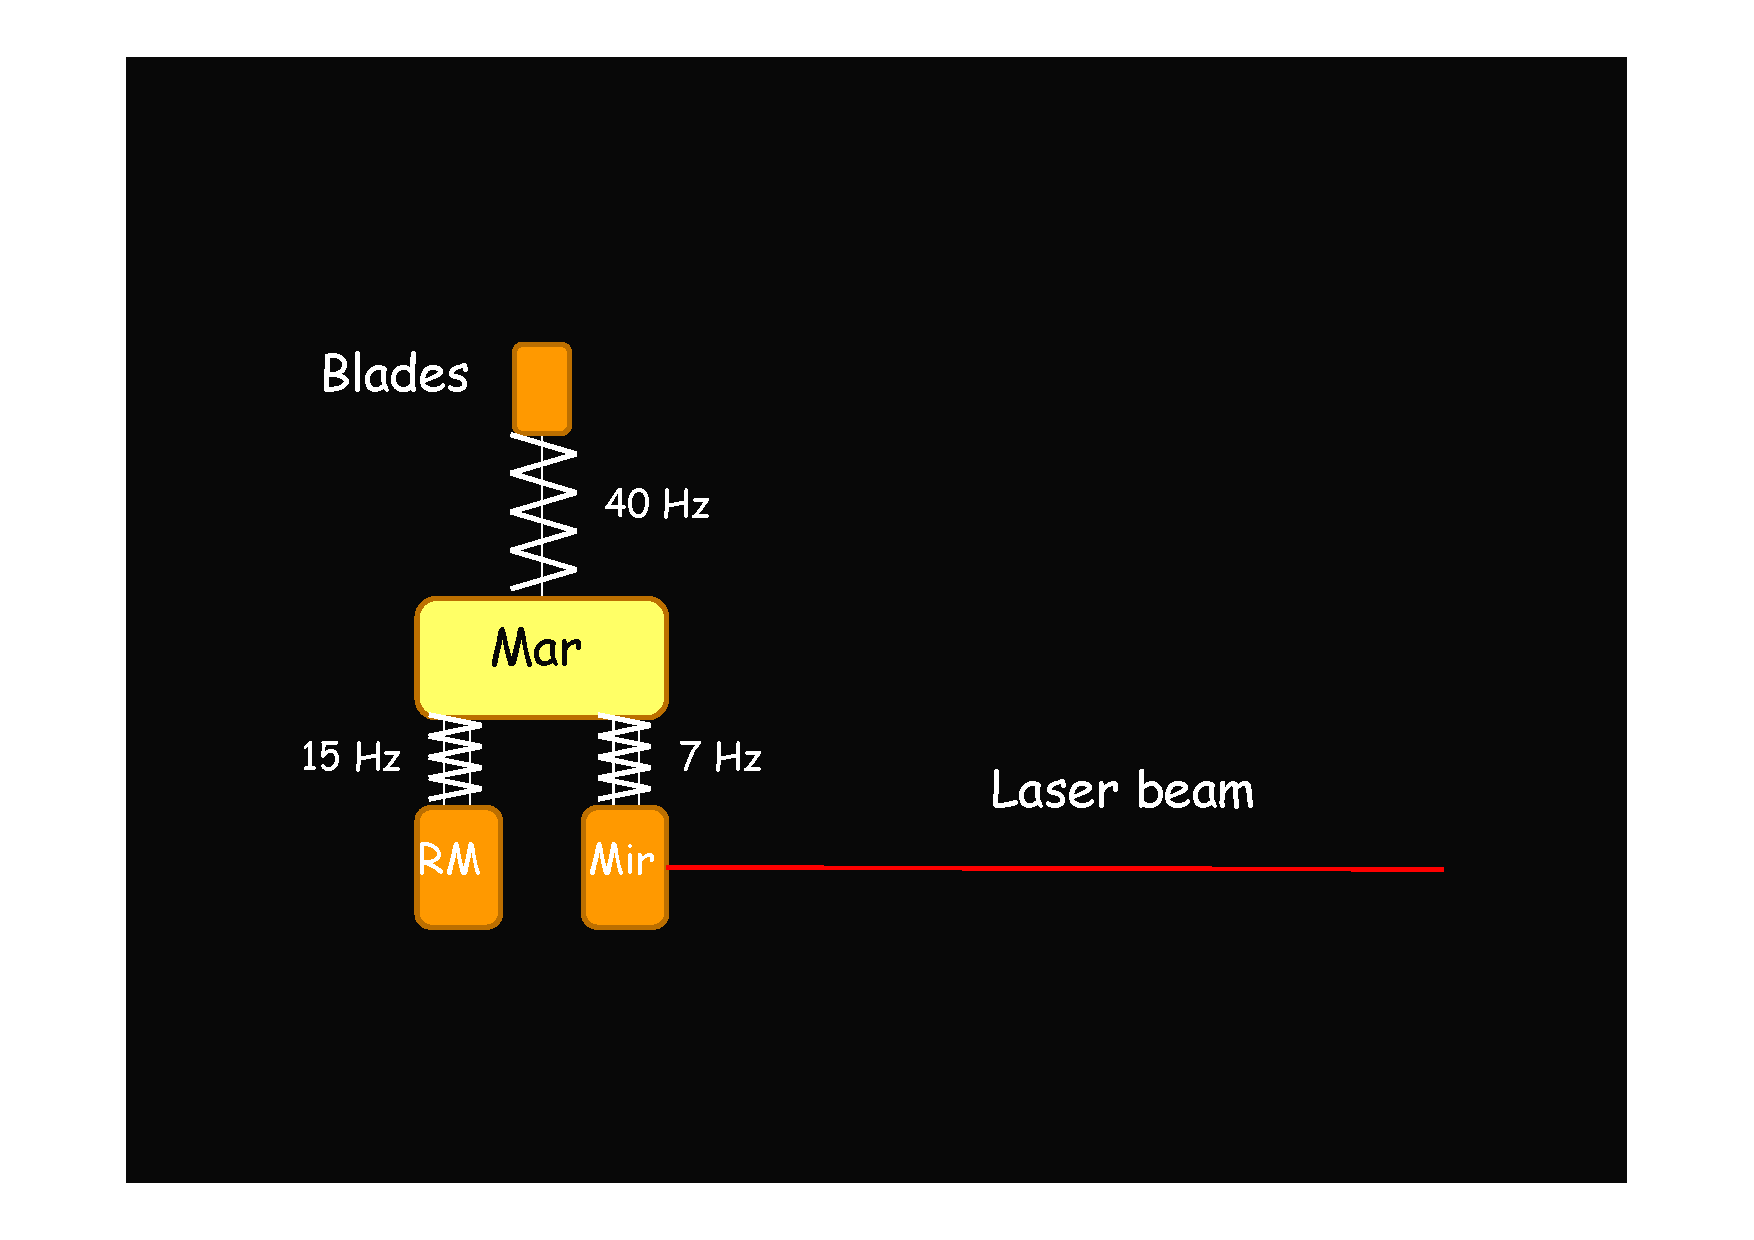
\includegraphics[width=13cm]{./Sec_Suspensions/Figures/Creep-Fig1.pdf}
			\caption{The three vertical modes of the optical payload suspended from the blades of last filter of the chain. For the vertical dynamics the two thin wires in a cradle configuration suspending the reference mass and the mirror can be thought as single vertical springs. As mentioned in the text, the vertical normal modes involve mainly (but not only) displacements of each payload element suspended from the blades: Marionette (\emph{Mar}~-- 40\,Hz), Reference Mass (\emph{RM}~-- 15\,Hz) and Mirror (\emph{Mir}~-- 7\,Hz).}
\label{CFig1}
	\end{center}
\end{figure}
As sketched in Fig.~\ref{CFig1}, the dynamics of the optical payload along the vertical axis can be seen as the motion of three rigid bodies (mirror, reference mass and marionette) connected by three constraints (suspension wires). As a consequence, the payload vertical motion attached to the elastic blade spring of the last filter of the chain exhibits three fundamental modes along the vertical direction involving mainly (but not only) the vertical displacement of the reference mass, mirror and marionette respectively (see Fig.~\ref{CFig1}).
These vertical modes are well visible on the Virgo interferometer output port, namely they appear as peaks on the output photo-diode placed in front of the detector dark fringe (see Fig.~\ref{CFig2}). This means that the modes are excited by some spurious vertical force of unknown origin. 
\begin{figure}[t]
	\begin{center}
		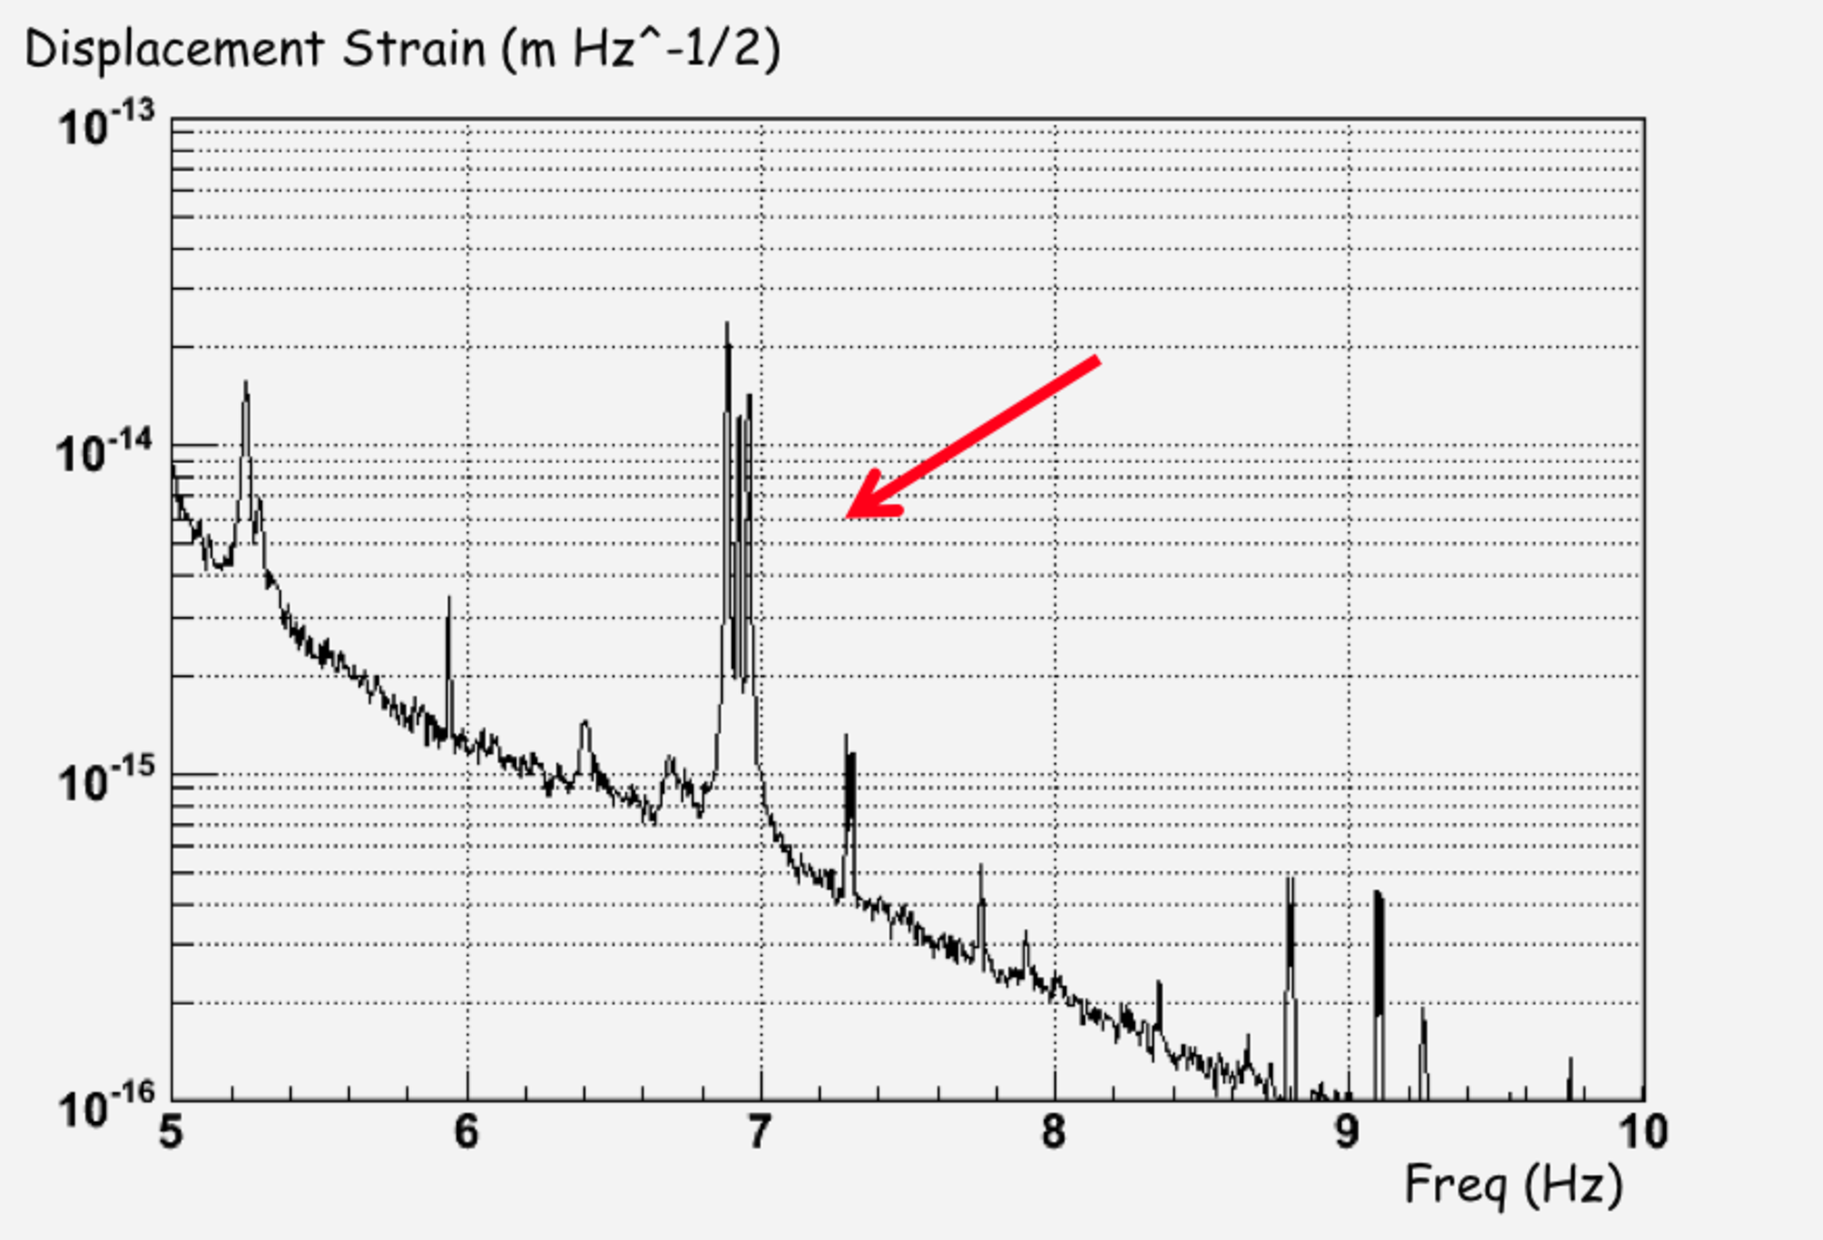
\includegraphics[width=13cm]{./Sec_Suspensions/Figures/Creep-Fig2.pdf}
			\caption{The photo-diode signal at the dark port of the Virgo antenna expressed in strain sensitivity. The four peaks around 7\,Hz correspond to the vertical modes where the mirror displacement is mainly involved. A peak for each one of the four mirrors accommodated along the two Fabry-Perot cavities appears in the dark port (each at a slight different frequency around 7\,Hz).}
\label{CFig2}
	\end{center}
\end{figure}
The micro-creep, such as thermal noise or the electro-mechanical noise floor coming from the coil-magnet actuators are only possible excitation mechanisms. Using the coil-magnet actuators steering the marionette it is possible to excite the three vertical normal modes of the payload. More in general, it is possible to measure the transfer function between the vertical force acting on the marionette and the mirror longitudinal displacement (measured with very high accuracy by the Virgo interferometer). 
\begin{figure}[t]
	\begin{center}
		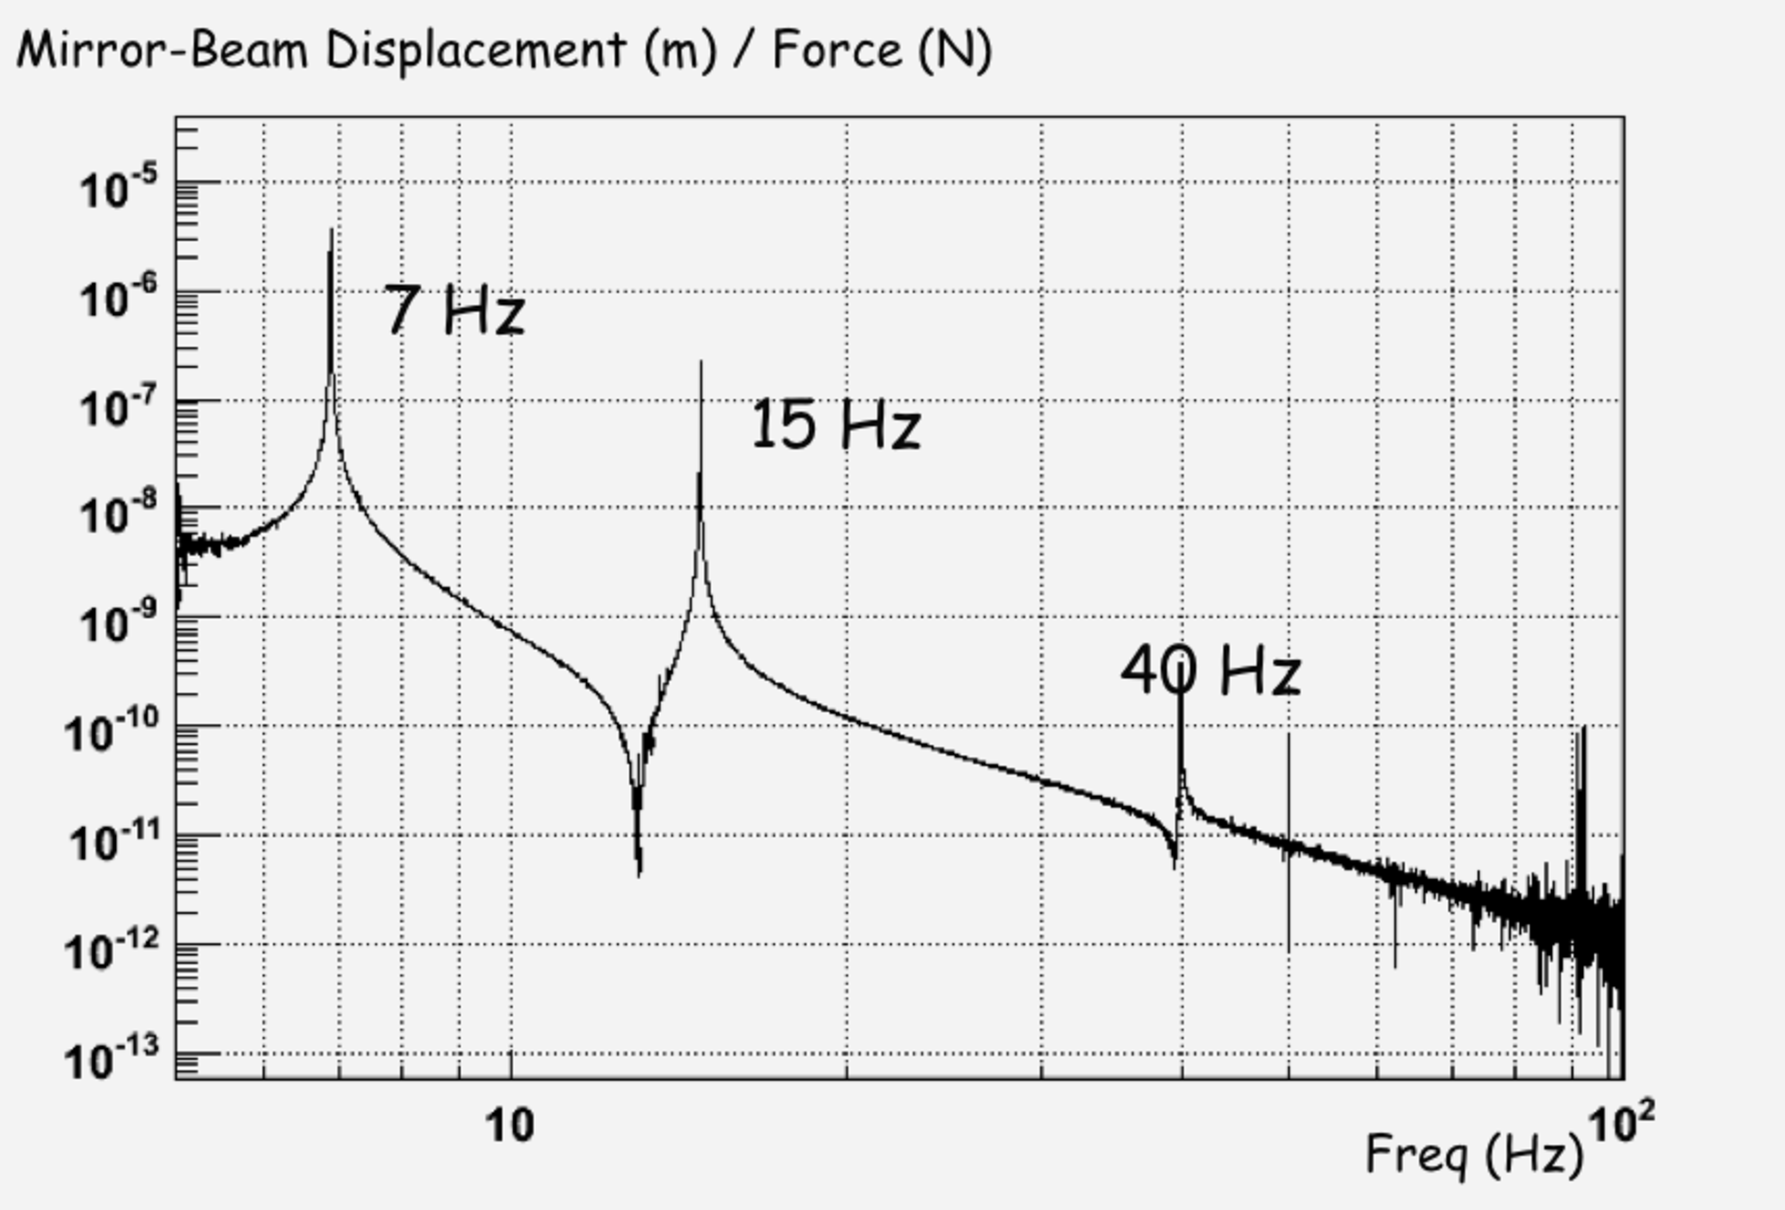
\includegraphics[width=15cm]{./Sec_Suspensions/Figures/Creep-Fig3.pdf}
			\caption{The transfer function between the mirror displacement along the beam (expressed in m) and the vertical force acting on the marionette (expressed in N). The vertical to horizontal coupling-factor (i.e.\ how much the mirror displacement in vertical is transmitted horizontally along the beam) is obviously already included in our measured transfer function and does not require any additional evaluation.}
\label{CFig3}
	\end{center}
\end{figure}
%%
\begin{figure}[t]
	\begin{center}
		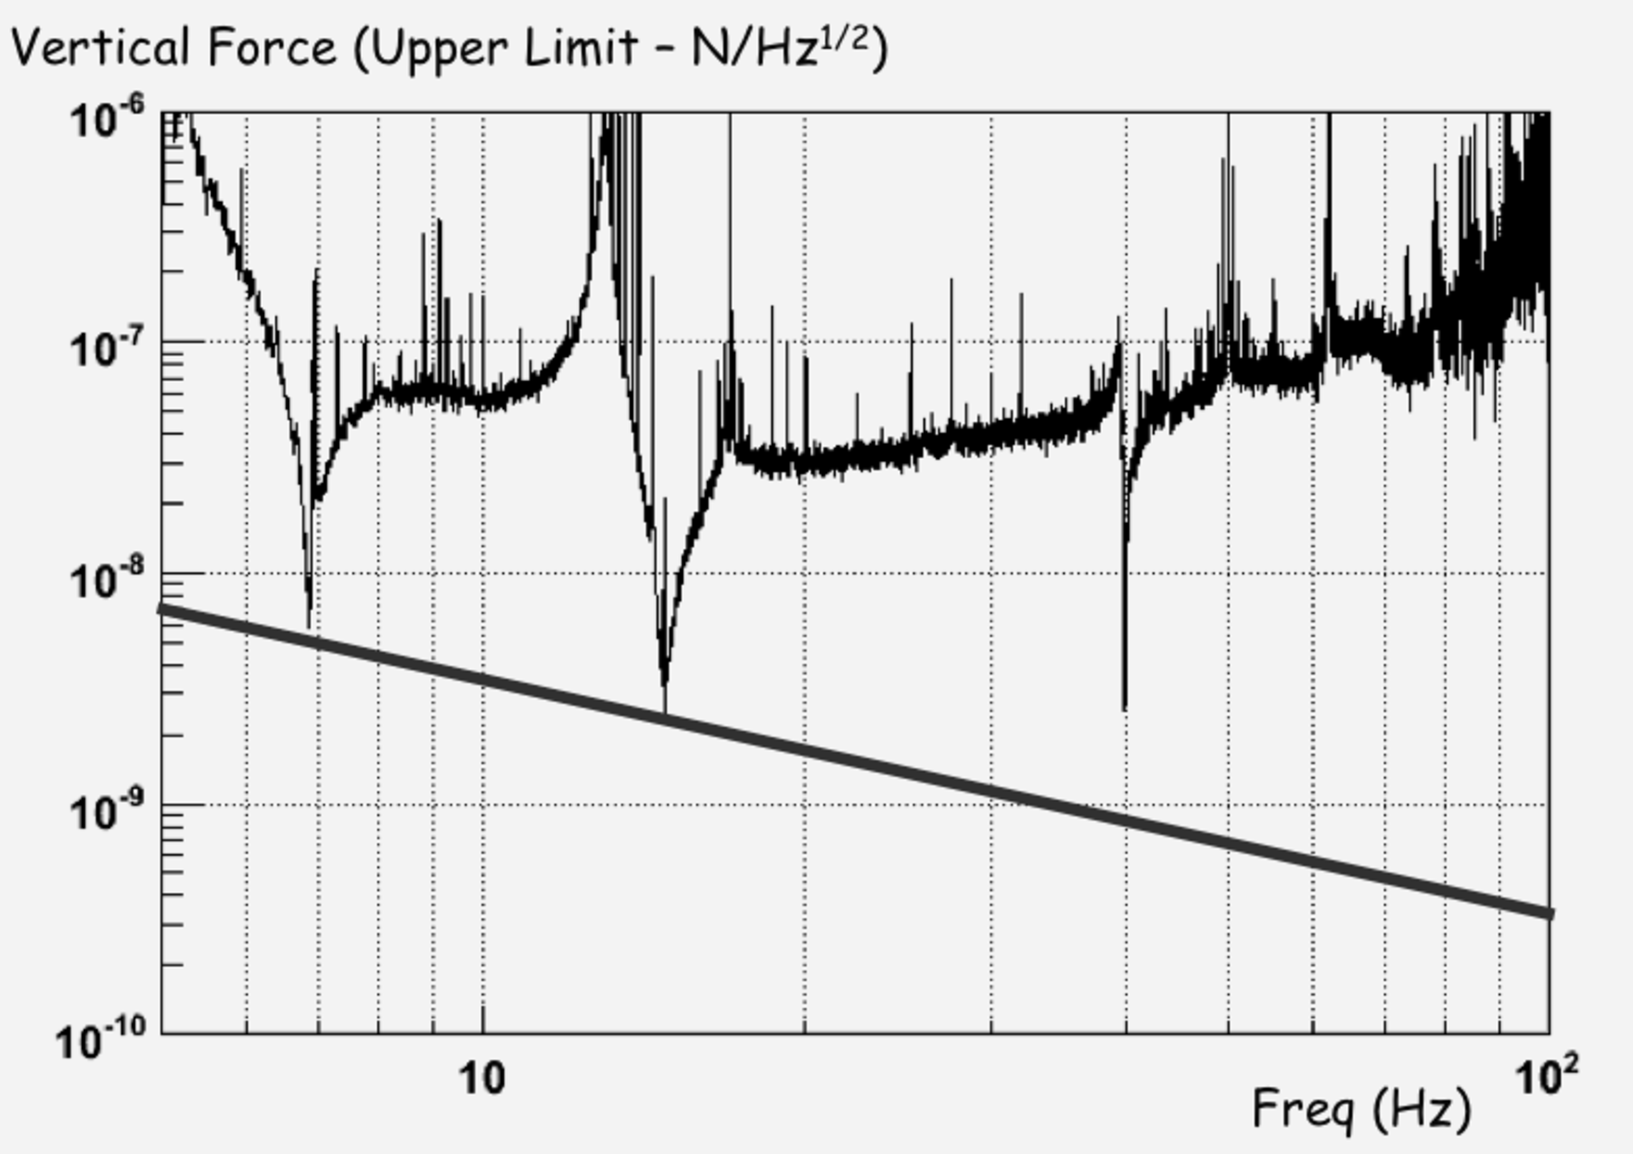
\includegraphics[width=15cm]{./Sec_Suspensions/Figures/Creep-Fig4.pdf}
			\caption{The linear spectral density of the maximum possible vertical force acting on the marionette compatible with the Virgo sensitivity. This is given by the simple procedure described in the text. Since the ``$1/f$-behavior'' of the micro-glitches force is assumed, one can find what is the maximum force having an ``$1/f$-profile'' at the level of the marionette compatible with the Virgo sensitivity. This is given by the minimal ``$1/f$-shape'' line touching the curve that gives the general upper limit on the vertical force just plotted. }
\label{CFig4}
	\end{center}
\end{figure}
%%
\begin{figure}[t]
	\begin{center}
		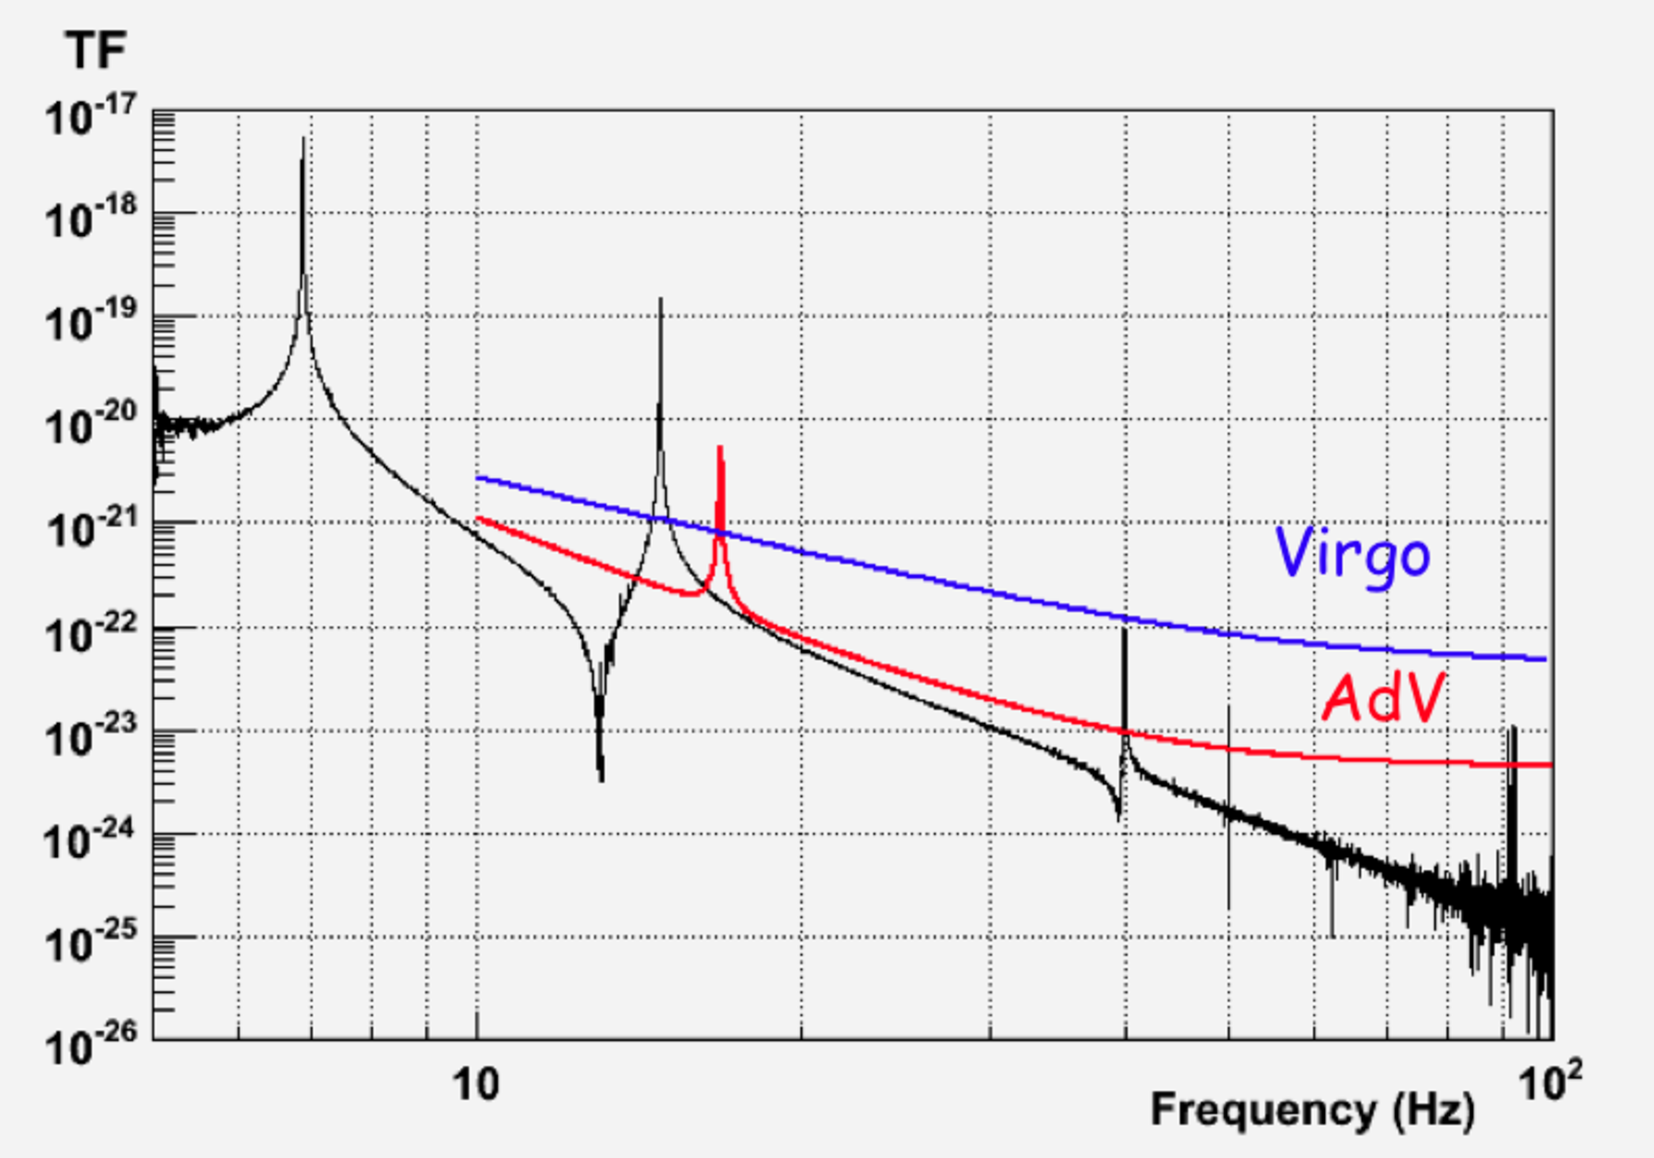
\includegraphics[width=15cm]{./Sec_Suspensions/Figures/Creep-Fig5.pdf}
			\caption{The upper limit of the micro-creep noise floor taking place in vertical on the blades of the last stage is given by the ``$1/f$-force'' upper limit plotted in the previous figure and the mentioned transfer function (stating how this force is transmitted along the beam). The upper limit of this noise floor is compared with the design sensitivity curves of Virgo and AdV. The upper limit, except around the resonant peaks, is enough to state that AdV will not be affected by this source of noise.}
\label{CFig5}
	\end{center}
\end{figure}
%%
The measured transfer function (mirror displacement along the beam, expressed in m over the vertical force applied on the marionette, expressed in N) is plotted in Fig.~\ref{CFig3}. In order to set an upper limit on the vertical force presently acting on the marionette, one can make the ultra-conservative hypothesis (likely not realistic) that the vertical spurious force is dominant in all the band, namely it is responsible of the present sensitivity of the detector. With this assumption, dividing the present sensitivity (expressed in displacement along the beam) by the mentioned transfer function (mirror displacement vs.\ vertical force) the linear spectral density of the maximum vertical force acting on the marionette compatible with the measured sensitivity can be plotted (see Fig.~\ref{CFig4}). 
The deeps due to the three vertical modes of the payload (where the denominator - the transfer function - is large because of the resonant frequencies) are well visible. As mentioned above, the micro-glitches are expected to induce a shot-noise, namely a ``$1/f$-colored force'' thus one can set also the maximum ``$1/f$-like force'' compatible with the present sensitivity (see line at Fig.~\ref{CFig4}). By multiplying the plotted $1/f$-force by the measured transfer function (mirror displacement divided by vertical force on the marionette) one can thus obtain the linear spectral density of the maximum displacement induced by the micro-glitches on the mirror. This upper limit is compared in Fig.~\ref{CFig5} with the sensitivity of the Virgo and AdV. From this figure, one can see that the upper limit just set is sufficient to exclude a dominant contribution in AdV. An important remark is that the micro-glitches are expected to increase when the operation vertical frequency of the anti-seismic filters is reduced. On the other hand, as described in section 4.1.1d, we know that working with seismic filters tuned around 300\,mHz is a must to achieve the required vertical attenuation in the Einstein Telescope. However, several last filters of the \emph{Superattenuator} chains are already working around 300\,mHz and thus our result, excluding a dominant effect due to micro-glitches in Advanced detectors at the level of last filter blades , is valid also at this tuning frequency. The present upper limit is thus surely valid also in Einstein Telescope. On the other hand this upper limit is far (several orders of magnitude) from the third generation sensitivity, especially in the ultra-low frequency range. Since the micro-glitches of the elastic blades taking place on the upper stages of the chain are strongly filtered by the anti-seismic filter underneath, it is obvious that possible problems coming from micro-glitches (if present) can affect the sensitivity of the third generation antenna only if they take place at the level of the last filter(s) of the chain. 
A dedicated R\&D programme to minimize micro-glitch effects on the cryogenic payload (see Appendix) and, if necessary, on the last stage(s) of the \emph{Superattenuator}, is mandatory. In any case this is not expected to affect our anti-seismic isolation strategy, at least on the upper isolation chains.

\paragraph{f) SA control strategy and improvements for ET}

The Suspension Control System plays a crucial role in the interferometer operation. At the top level, it provides DC positioning control and damping of chain normal modes along horizontal, vertical and yaw degrees of freedom. At the bottom it provides the handle to apply residual correction from ground onto the horizontal and yaw degrees of freedom through the steering filter usually left actuation-free. Given the payload suspension point controlled with suitable accuracy, another section of the control is devoted to apply internal forces to the payload and to the interferometer control. The overall structure, described by more than 80 vibrational modes model, is presently (Virgo/Virgo+) controlled by 18 coil-magnet pairs actuators while its status is monitored by using about 20 sensors.

Such controls make use of two main classes of error signals: \emph{local controls} and \emph{global controls}. Local controls use error signals generated by local sensors, accommodated on or close to the suspension structure. Global controls are those whose input signal is generated by sensors located "far" from the suspension mechanics or traced by the interferometer signal. Typical local control sensors are accelerometer located on suspension and position sensors measuring displacement between suspension and suspension enclosure like linear variable differential transformers (\emph{LVDT}). For the payload local control CCD cameras and PSD optical levers are used. Usual global control sensors are photo-diodes or quadrant photo-diodes providing information on suspended optical elements along three directions related to the interferometer beam (longitudinal displacement and two transverse tilts).

In order to ensure drift-less control and to provide suitable response of the system during far earthquakes, with the Virgo set-up, remote sensors and interferometer signals are combined with local sensors. Significant examples are the drift-less local control of mirrors alignment and the Global Inverted-Pendulum Control (\emph{GIPC}). Long suspensions in their \emph{rest} position, without any applied force, are usually up to a several millimetres far from their nominal working point. For this reason the control system has a large dynamics, i.e. it  is able to control over several order of magnitude, and this task is accomplished by using suitable large dynamics sensors and actuators. Once the RMS accuracy of the suspension point (at the top of the mechanical structure) is brought to $\sim 0.1\,\mathrm{\mu m}$, large angular oscillations or DC misalignment can still be present at the level of the payload and local controls are engaged to slow down mirror motion to $\sim 1\,\mathrm{\mu m /s}$ while aligning it from $50\,\mathrm{\mu\text{rad}}$ down to 10\,nrad accuracy. 
In section~\ref{sec:last_stage} some specific issues involving local controls of the payload will be further commented. In fact for ET the role played by the payload and its controls will be crucial in the overall suspension performance even more critically than for Virgo.

In Virgo we successfully tested multi-dynamical range actuators, to apply locking force through the payloads, which are capable of switching between operational modes without introducing discontinuities in the feedback. Meeting injected noise requirements should not be an issue using such devices. To cover the whole huge dynamical range actuation forces are distributed along the chain. In the case of the ET suspension, whatever will be its  final mechanical design,  it seems that we cannot use less than  four actuation points (presently inverted pendulum, steering filter, marionette and mirror). 

Digital controllers used in suspension control system are quite complex: about 250 poles for each suspension requiring about 150 $MFLOPS$ computation capabilities (sustained). One of the key points for a second generation system will be providing tools to ease control engineers life. Today control loops performances are a function of who actually implements the control algorithm. In the past this approach showed to slowly converge to a nearly optimal control. The present evolution of this techniques allows optimal control using almost automated procedures 
much more human independent than $Nyquist$ like approach used so far.
%
\subsubsection{HF interferometer}

As detailed in section 4.1.1.c, the measurements campaign performed with the Virgo interferometer and devoted to evaluate the attenuation performance of the \emph{Superattenuator}, demonstrated that, above 3 Hz, a multistage pendulum suspended to a three legs mechanical structure, as pre-isolator stage, is compliant with the ET requirements. The results reported in figure~\ref{FigSusp5} have been obtained by using a \emph{Superattenuator} 
with \emph{six} seismic filters (for a total length of about 9\,m) hung to a platform accommodated on top of the Inverted Pendulum which has been by-passed during the suspension point excitation phase of the measurements. This represents a good safety margin from attenuation point of view, because passing the seismic noise through the mechanical structure of the Inverted Pendulum, it will be additionally attenuated by a factor around 20--40\,dB.

Starting from the long experience acquired in operating a similar mechanical system for seismic noise suppression, a base line for the LF and HF Detectors of the ET Project has been tracked. It is based a seismic attenuation system designed for the Virgo interferometer with common peculiarities: the first one can be conceived extending the detection bandwidth below 3 Hz by improving the chain total length up to 17\,m , while for the second a Virgo-like \emph{Superattenuator} can be built. The advantages of this choice are different:  
\begin{itemize}
\item even considering a conservative cut-off frequency of the whole system around 5\,Hz, it turns out that there will be a wide overlap between the HF Interferometer bandwidth the LF Interferometer one (following our indication starting around 2\,Hz);
\item the construction technology, mainly based on the use of magnetic anti-spring, has been deeply tested in vacuum for a very long time period (about ten years);
\item the behavior of high stressed elastic elements (blades and wires) has been 
studied;
\item many mechanical and electro-mechanical elements are compatible with cryogenic environment (see the Appendix \ref{sec:cryo_filters});
\item the upgrades, presently in progress for the Virgo \emph{Superattenuator}, 
can be used for this application too.
\end{itemize}

In this context and considering the ET requirements the choice of the Virgo \emph{Superattenuator} as seismic isolation system for the third generation of gravitational wave detector,seems to be the natural one.

\FloatBarrier 

\longetbox{r}{box:Final}{Final considerations on Suspension for ET-LF and ET-HF}
{ 
\begin{itemize}
\item Above 3 Hz the present Virgo \emph{Superattenuator} is compliant with the ET requirements. Minor changes are needed to extend the detection bandwidth in the low frequency region (below 3Hz). The \emph{Superattenuator} is a very good candidate to be installed in the \emph {LF Interferometer} for the following reasons:
	\begin{itemize}
	\item it has well tested behavior over 10 years activity;
	\item it has well tested technology;
	\item vacuum compatibility of crucial elements (under vacuum for many years);
	\item many mechanical and electro-mechanical elements compatible with cryogenic environment.
	\end{itemize}
\item A \emph{Superattenuator} 17 m tall with six stages (filters) in "equal-spaced" configuration and filter tuning (using the magnetic anti-spring) with a vertical cut-off around 300 mHz represents the reference solution for the ET Project. With this set-up a suspension system with a conservative cross-over frequency around 1.8 Hz (compliant with ET requirements) can be built.
\item The Virgo \emph{Superattenuator} could be used as seismic isolation system of the \emph {HF Interferometer} for the following reasons:
	\begin{itemize}
		\item the attenuation performance is compliant with the ET requirements;
		\item the cross-over frequency (around 5 Hz) is good for this purpose;
		\item the technology used (magnetic anti-spring filters) for its construction is well tested ;
		\item all the upgrades of the system, presently in progress, are available also for this application.
	\end{itemize}
\item Ten years of activity on the control system of the \emph{Superattenuator} represents a clear demonstration that a feed-back control at low-noise can be used to improve its performance in the low frequency region (below 5 Hz). The acquired experience on this subject is a valuable starting point for the commissioning of next generation detectors.
\item The construction of the seismic isolation systems for Einstein Telescope could start immediately after a slight refinement of the project. Thanks to the Virgo experience the \emph{Superattenuator}, developed to filter seismic noise at the mirror level, is the reference solution for the project.
\end{itemize}
}
%%%
\subsubsection{Upper-lower suspension interface}
\label{Upper_lower_suspension_interface}

As described all along this document, the ET Project is based on two different detectors. The first one aimed to the detection of gravitational wave signals in the low frequency range (\emph{LF Interferometer}) and the second one for the detection of high frequency signals (\emph{HF Interferometer}). The LF experimental apparatus will have a detection bandwidth as wide as possible in this specific region adopting, as seismic isolation system, the Virgo \emph{Superattenuator}. The main difference is represented by the length of the multistage pendulum (for details see section 4.1.1.d), an important parameter to move the cut-off frequency of the whole system to the best value in accordance with the ET requirements (around 2 Hz for a total chain length of about 17\,m).
The main characteristic of the LF Detector is that the suspension upper part will be at room temperature while the payload is maintained at cryogenic temperature for beating the thermal noise limit. These working conditions will not be present in the HF Detector where a seismic isolation system based on the Virgo \emph{Superattenuator} 9\,m high will be operated at room temperature thanks to its attenuation performance above 3\,Hz compliant with the ET requirements. 

For this project a complex vacuum system has been studied with both interferometers within the same tunnel and in particular with the pipes for LF Interferometer running on top of those ones of the HF Detector. This configuration will include a cooling shield containing the payload within the vacuum tower basement of the LF Interferometer. While the test mass and the penultimate stage of the suspension will be accommodated within the cryostat, a suspension wire made of Ti-6Al-4V will be used to suspend the payload from the \emph{Superattenuator} upper part at room temperature (see section 3.4). This interconnection element has a key role in preserving the thermal isolation between the payload and the suspension upper part. Moreover, the cryostat structure will have a hole through which this suspension wire will pass. This hole should be large enough to avoid possible wire friction during standard working condition, but it should not create an important and undesirable thermal input for the cryostat operation. The penultimate stage, indeed, will be directly connected through a thermal link to an ancillary suspension where a \emph{cold box} will be installed. In this way the heat extraction from the mirror is obtained via the suspension fibres attached to the penultimate stage, and then through the thermal link toward the ancillary suspension.

Since the hole in the cryostat structure will be also used for pure helium gas exchange during the cooling down process (pure helium gas will be injected within the experimental volume to speed up the cooling down/warming up procedure), it will be equipped with a mechanical shutter (vacuum tight) driven by a stepping motor (remotely controlled for opening/closing procedure) to be installed in the roof structure separating the tower upper part from the bottom one. This mechanical solution together with an adequate pumping system and a well defined evacuation procedure will be important steps to reach the needed vacuum level. 

